\documentclass[]{article}
\usepackage{lmodern}
\usepackage{amssymb,amsmath}
\usepackage{ifxetex,ifluatex}
\usepackage{fixltx2e} % provides \textsubscript
\ifnum 0\ifxetex 1\fi\ifluatex 1\fi=0 % if pdftex
  \usepackage[T1]{fontenc}
  \usepackage[utf8]{inputenc}
\else % if luatex or xelatex
  \ifxetex
    \usepackage{mathspec}
  \else
    \usepackage{fontspec}
  \fi
  \defaultfontfeatures{Ligatures=TeX,Scale=MatchLowercase}
\fi
% use upquote if available, for straight quotes in verbatim environments
\IfFileExists{upquote.sty}{\usepackage{upquote}}{}
% use microtype if available
\IfFileExists{microtype.sty}{%
\usepackage{microtype}
\UseMicrotypeSet[protrusion]{basicmath} % disable protrusion for tt fonts
}{}
\usepackage[margin=1in]{geometry}
\usepackage{hyperref}
\hypersetup{unicode=true,
            pdftitle={Linear model fit for p-value discrepancies},
            pdfborder={0 0 0},
            breaklinks=true}
\urlstyle{same}  % don't use monospace font for urls
\usepackage{color}
\usepackage{fancyvrb}
\newcommand{\VerbBar}{|}
\newcommand{\VERB}{\Verb[commandchars=\\\{\}]}
\DefineVerbatimEnvironment{Highlighting}{Verbatim}{commandchars=\\\{\}}
% Add ',fontsize=\small' for more characters per line
\usepackage{framed}
\definecolor{shadecolor}{RGB}{248,248,248}
\newenvironment{Shaded}{\begin{snugshade}}{\end{snugshade}}
\newcommand{\KeywordTok}[1]{\textcolor[rgb]{0.13,0.29,0.53}{\textbf{#1}}}
\newcommand{\DataTypeTok}[1]{\textcolor[rgb]{0.13,0.29,0.53}{#1}}
\newcommand{\DecValTok}[1]{\textcolor[rgb]{0.00,0.00,0.81}{#1}}
\newcommand{\BaseNTok}[1]{\textcolor[rgb]{0.00,0.00,0.81}{#1}}
\newcommand{\FloatTok}[1]{\textcolor[rgb]{0.00,0.00,0.81}{#1}}
\newcommand{\ConstantTok}[1]{\textcolor[rgb]{0.00,0.00,0.00}{#1}}
\newcommand{\CharTok}[1]{\textcolor[rgb]{0.31,0.60,0.02}{#1}}
\newcommand{\SpecialCharTok}[1]{\textcolor[rgb]{0.00,0.00,0.00}{#1}}
\newcommand{\StringTok}[1]{\textcolor[rgb]{0.31,0.60,0.02}{#1}}
\newcommand{\VerbatimStringTok}[1]{\textcolor[rgb]{0.31,0.60,0.02}{#1}}
\newcommand{\SpecialStringTok}[1]{\textcolor[rgb]{0.31,0.60,0.02}{#1}}
\newcommand{\ImportTok}[1]{#1}
\newcommand{\CommentTok}[1]{\textcolor[rgb]{0.56,0.35,0.01}{\textit{#1}}}
\newcommand{\DocumentationTok}[1]{\textcolor[rgb]{0.56,0.35,0.01}{\textbf{\textit{#1}}}}
\newcommand{\AnnotationTok}[1]{\textcolor[rgb]{0.56,0.35,0.01}{\textbf{\textit{#1}}}}
\newcommand{\CommentVarTok}[1]{\textcolor[rgb]{0.56,0.35,0.01}{\textbf{\textit{#1}}}}
\newcommand{\OtherTok}[1]{\textcolor[rgb]{0.56,0.35,0.01}{#1}}
\newcommand{\FunctionTok}[1]{\textcolor[rgb]{0.00,0.00,0.00}{#1}}
\newcommand{\VariableTok}[1]{\textcolor[rgb]{0.00,0.00,0.00}{#1}}
\newcommand{\ControlFlowTok}[1]{\textcolor[rgb]{0.13,0.29,0.53}{\textbf{#1}}}
\newcommand{\OperatorTok}[1]{\textcolor[rgb]{0.81,0.36,0.00}{\textbf{#1}}}
\newcommand{\BuiltInTok}[1]{#1}
\newcommand{\ExtensionTok}[1]{#1}
\newcommand{\PreprocessorTok}[1]{\textcolor[rgb]{0.56,0.35,0.01}{\textit{#1}}}
\newcommand{\AttributeTok}[1]{\textcolor[rgb]{0.77,0.63,0.00}{#1}}
\newcommand{\RegionMarkerTok}[1]{#1}
\newcommand{\InformationTok}[1]{\textcolor[rgb]{0.56,0.35,0.01}{\textbf{\textit{#1}}}}
\newcommand{\WarningTok}[1]{\textcolor[rgb]{0.56,0.35,0.01}{\textbf{\textit{#1}}}}
\newcommand{\AlertTok}[1]{\textcolor[rgb]{0.94,0.16,0.16}{#1}}
\newcommand{\ErrorTok}[1]{\textcolor[rgb]{0.64,0.00,0.00}{\textbf{#1}}}
\newcommand{\NormalTok}[1]{#1}
\usepackage{graphicx,grffile}
\makeatletter
\def\maxwidth{\ifdim\Gin@nat@width>\linewidth\linewidth\else\Gin@nat@width\fi}
\def\maxheight{\ifdim\Gin@nat@height>\textheight\textheight\else\Gin@nat@height\fi}
\makeatother
% Scale images if necessary, so that they will not overflow the page
% margins by default, and it is still possible to overwrite the defaults
% using explicit options in \includegraphics[width, height, ...]{}
\setkeys{Gin}{width=\maxwidth,height=\maxheight,keepaspectratio}
\IfFileExists{parskip.sty}{%
\usepackage{parskip}
}{% else
\setlength{\parindent}{0pt}
\setlength{\parskip}{6pt plus 2pt minus 1pt}
}
\setlength{\emergencystretch}{3em}  % prevent overfull lines
\providecommand{\tightlist}{%
  \setlength{\itemsep}{0pt}\setlength{\parskip}{0pt}}
\setcounter{secnumdepth}{0}
% Redefines (sub)paragraphs to behave more like sections
\ifx\paragraph\undefined\else
\let\oldparagraph\paragraph
\renewcommand{\paragraph}[1]{\oldparagraph{#1}\mbox{}}
\fi
\ifx\subparagraph\undefined\else
\let\oldsubparagraph\subparagraph
\renewcommand{\subparagraph}[1]{\oldsubparagraph{#1}\mbox{}}
\fi

%%% Use protect on footnotes to avoid problems with footnotes in titles
\let\rmarkdownfootnote\footnote%
\def\footnote{\protect\rmarkdownfootnote}

%%% Change title format to be more compact
\usepackage{titling}

% Create subtitle command for use in maketitle
\providecommand{\subtitle}[1]{
  \posttitle{
    \begin{center}\large#1\end{center}
    }
}

\setlength{\droptitle}{-2em}

  \title{Linear model fit for p-value discrepancies}
    \pretitle{\vspace{\droptitle}\centering\huge}
  \posttitle{\par}
    \author{}
    \preauthor{}\postauthor{}
    \date{}
    \predate{}\postdate{}
  

\begin{document}
\maketitle

\begin{Shaded}
\begin{Highlighting}[]
\CommentTok{#rasq = read.csv("linear_model_cov.csv")}
\NormalTok{rasq =}\StringTok{ }\KeywordTok{read.csv}\NormalTok{(}\StringTok{"linear_model_cov_upd.csv"}\NormalTok{)}
\NormalTok{rasq =}\StringTok{ }\NormalTok{rasq[}\OperatorTok{!}\KeywordTok{is.na}\NormalTok{(rasq}\OperatorTok{$}\NormalTok{pvalT),]}
\KeywordTok{dim}\NormalTok{(rasq)}
\end{Highlighting}
\end{Shaded}

\begin{verbatim}
## [1] 13978    32
\end{verbatim}

\begin{Shaded}
\begin{Highlighting}[]
\NormalTok{rasq[}\DecValTok{1}\OperatorTok{:}\DecValTok{2}\NormalTok{,]}
\end{Highlighting}
\end{Shaded}

\begin{verbatim}
##                  fID                      sID SNPchr    SNPpos Ref Alt
## 1 ENSG00000000457.11 rs12132222:169758564:A:G   chr1 169789423   A   G
## 2 ENSG00000000938.10               rs12732199   chr1  27669961   G   A
##         AF HWEChisq impQual       qval      Chi2       Pi DeltaErr
## 1 0.069643 1.568960       1 -1.7307995  8.946188 0.522254 0.000799
## 2 0.253571 2.488767       1 -0.5920312 11.183474 0.437893 0.000420
##    PhiBias        OD NfSNP NrSNP  corfSNP  corrSNP      qvalT    pvalT
## 1 0.490439 32.119716    23  1443 0.993050 0.967369 0.06476087 0.000264
## 2 0.427457  5.554724     1   310 0.907844 0.990352 0.11762400 0.000203
##         pvalR   odNB    odBB       mpp   asT   asR     pvalRupd
## 1 0.002780492 0.0344 0.00136 0.3168056 12282 13382 4.371877e-04
## 2 0.000825291 0.1860 0.04200 0.4875028  2788   409 6.291182e-05
##          ODupd pvalTupd odNBupd odBBupd
## 1 1.827724e-10  0.00189  0.0267 0.00139
## 2 3.325598e-03  0.00022  0.1100 0.08180
\end{verbatim}

\begin{Shaded}
\begin{Highlighting}[]
\NormalTok{rasq}\OperatorTok{$}\NormalTok{qvalR =}\StringTok{ }\DecValTok{10}\OperatorTok{^}\NormalTok{rasq}\OperatorTok{$}\NormalTok{qval}
\NormalTok{rasq}\OperatorTok{$}\NormalTok{qvalT[rasq}\OperatorTok{$}\NormalTok{qvalT}\OperatorTok{<}\FloatTok{1e-100}\NormalTok{] =}\StringTok{ }\FloatTok{1e-100}
\NormalTok{rasq}\OperatorTok{$}\NormalTok{qvalR[rasq}\OperatorTok{$}\NormalTok{qvalR}\OperatorTok{<}\FloatTok{1e-100}\NormalTok{] =}\StringTok{ }\FloatTok{1e-100}
\NormalTok{rasq}\OperatorTok{$}\NormalTok{pvalT[rasq}\OperatorTok{$}\NormalTok{pvalT}\OperatorTok{<}\FloatTok{1e-100}\NormalTok{] =}\StringTok{ }\FloatTok{1e-100}
\NormalTok{rasq}\OperatorTok{$}\NormalTok{pvalR[rasq}\OperatorTok{$}\NormalTok{pvalR}\OperatorTok{<}\FloatTok{1e-100}\NormalTok{] =}\StringTok{ }\FloatTok{1e-100}
\KeywordTok{dim}\NormalTok{(rasq)}
\end{Highlighting}
\end{Shaded}

\begin{verbatim}
## [1] 13978    33
\end{verbatim}

\begin{Shaded}
\begin{Highlighting}[]
\CommentTok{#rasq$rnlt = -log10(rasq$qvalR)}
\CommentTok{#rasq$tnlt = -log10(rasq$qvalT)}

\CommentTok{#rasq$rnlt = -log10(rasq$pvalR)}
\CommentTok{#rasq$tnlt = -log10(rasq$pvalT)}

\NormalTok{rasq}\OperatorTok{$}\NormalTok{rnlt =}\StringTok{ }\OperatorTok{-}\KeywordTok{log10}\NormalTok{(rasq}\OperatorTok{$}\NormalTok{pvalRupd)}
\NormalTok{rasq}\OperatorTok{$}\NormalTok{tnlt =}\StringTok{ }\OperatorTok{-}\KeywordTok{log10}\NormalTok{(rasq}\OperatorTok{$}\NormalTok{pvalTupd)}
\NormalTok{rasq =}\StringTok{ }\NormalTok{rasq[}\OperatorTok{!}\KeywordTok{is.na}\NormalTok{(rasq}\OperatorTok{$}\NormalTok{pvalTupd),]}

\NormalTok{cent =}\StringTok{ }\ControlFlowTok{function}\NormalTok{(x)\{}
\NormalTok{  med =}\StringTok{ }\KeywordTok{median}\NormalTok{(x)}
\NormalTok{  (x}\OperatorTok{-}\NormalTok{med)}
\NormalTok{\}}
\NormalTok{norm =}\StringTok{ }\ControlFlowTok{function}\NormalTok{(x)\{}
\NormalTok{  sd =}\StringTok{ }\KeywordTok{sd}\NormalTok{(x)}
\NormalTok{  x}\OperatorTok{/}\NormalTok{sd}
\NormalTok{\}}

\NormalTok{odNB =}\StringTok{ }\NormalTok{rasq}\OperatorTok{$}\NormalTok{odNB; odNB[odNB}\OperatorTok{<}\FloatTok{1e-3}\NormalTok{]=}\FloatTok{1e-3}\NormalTok{; odNB[odNB}\OperatorTok{>}\DecValTok{8}\NormalTok{]=}\DecValTok{8}\NormalTok{; }
\NormalTok{odBB =}\StringTok{ }\NormalTok{rasq}\OperatorTok{$}\NormalTok{odBB; odBB[odBB}\OperatorTok{<}\FloatTok{1e-3}\NormalTok{]=}\FloatTok{1e-3}\NormalTok{; odBB[odBB}\OperatorTok{>}\DecValTok{8}\NormalTok{]=}\DecValTok{8}
\NormalTok{odR =}\StringTok{ }\NormalTok{rasq}\OperatorTok{$}\NormalTok{OD}
\NormalTok{lodNBp =}\StringTok{ }\KeywordTok{log10}\NormalTok{(odNB); }
\NormalTok{lodBBp =}\StringTok{ }\KeywordTok{log10}\NormalTok{(odBB); }
\NormalTok{lodRp =}\StringTok{ }\OperatorTok{-}\KeywordTok{log10}\NormalTok{(odR);}
\NormalTok{lodNB =}\StringTok{ }\KeywordTok{cent}\NormalTok{(}\KeywordTok{norm}\NormalTok{(lodNBp)); }
\NormalTok{lodBB =}\StringTok{ }\KeywordTok{cent}\NormalTok{(}\KeywordTok{norm}\NormalTok{(lodBBp)); }
\NormalTok{lodR =}\StringTok{ }\KeywordTok{cent}\NormalTok{(}\KeywordTok{norm}\NormalTok{(lodRp));}



\NormalTok{hiR =}\StringTok{ }\ControlFlowTok{function}\NormalTok{(cuts, y)\{}
\NormalTok{   kp =}\StringTok{ }\KeywordTok{abs}\NormalTok{(y)}\OperatorTok{>}\NormalTok{cuts}
   \KeywordTok{c}\NormalTok{(}\KeywordTok{mean}\NormalTok{(y[kp]}\OperatorTok{>}\DecValTok{0}\NormalTok{), }\KeywordTok{sum}\NormalTok{(kp)) }
\NormalTok{\}}
\CommentTok{#show RASQUAL }
\NormalTok{GfSNP =}\StringTok{ }\NormalTok{rasq}\OperatorTok{$}\NormalTok{NfSNP}
\NormalTok{GfSNP[rasq}\OperatorTok{$}\NormalTok{NfSNP}\OperatorTok{>}\DecValTok{1}\NormalTok{]=}\DecValTok{3}
\NormalTok{GfSNP[rasq}\OperatorTok{$}\NormalTok{NfSNP}\OperatorTok{>}\DecValTok{2}\NormalTok{]=}\DecValTok{6}
\NormalTok{GfSNP[rasq}\OperatorTok{$}\NormalTok{NfSNP}\OperatorTok{>}\DecValTok{4}\NormalTok{]=}\DecValTok{12}
\NormalTok{GfSNP[rasq}\OperatorTok{$}\NormalTok{NfSNP}\OperatorTok{>}\DecValTok{8}\NormalTok{]=}\DecValTok{24}
\NormalTok{GfSNP[rasq}\OperatorTok{$}\NormalTok{NfSNP}\OperatorTok{>}\DecValTok{16}\NormalTok{]=}\DecValTok{48}
\NormalTok{cutoff =}\StringTok{ }\DecValTok{25}
\NormalTok{rasq}\OperatorTok{$}\NormalTok{rnlt[rasq}\OperatorTok{$}\NormalTok{rnlt}\OperatorTok{>}\NormalTok{cutoff] =}\StringTok{ }\NormalTok{cutoff}
\NormalTok{rasq}\OperatorTok{$}\NormalTok{tnlt[rasq}\OperatorTok{$}\NormalTok{tnlt}\OperatorTok{>}\NormalTok{cutoff] =}\StringTok{ }\NormalTok{cutoff}
\NormalTok{y =}\StringTok{ }\NormalTok{rasq}\OperatorTok{$}\NormalTok{rnlt}\OperatorTok{-}\NormalTok{rasq}\OperatorTok{$}\NormalTok{tnlt}
\NormalTok{z =}\StringTok{ }\NormalTok{y}\OperatorTok{>}\DecValTok{0}
\NormalTok{kp0 =}\StringTok{ }\KeywordTok{abs}\NormalTok{(y)}\OperatorTok{>=}\DecValTok{0}
\NormalTok{kp1 =}\StringTok{ }\KeywordTok{abs}\NormalTok{(y)}\OperatorTok{>=}\DecValTok{1}
\NormalTok{kp5 =}\StringTok{ }\KeywordTok{abs}\NormalTok{(y)}\OperatorTok{>=}\DecValTok{5}
\NormalTok{kp10 =}\StringTok{ }\KeywordTok{abs}\NormalTok{(y)}\OperatorTok{>=}\DecValTok{10}
\NormalTok{kp15 =}\StringTok{ }\KeywordTok{abs}\NormalTok{(y)}\OperatorTok{>=}\DecValTok{15}

\NormalTok{ag0 =}\StringTok{ }\KeywordTok{aggregate}\NormalTok{(z[kp0], }\DataTypeTok{by=}\KeywordTok{list}\NormalTok{(GfSNP[kp0]), }\DataTypeTok{FUN=}\NormalTok{mean)}
\NormalTok{ag1 =}\StringTok{ }\KeywordTok{aggregate}\NormalTok{(z[kp1], }\DataTypeTok{by=}\KeywordTok{list}\NormalTok{(GfSNP[kp1]), }\DataTypeTok{FUN=}\NormalTok{mean)}
\NormalTok{ag5 =}\StringTok{ }\KeywordTok{aggregate}\NormalTok{(z[kp5], }\DataTypeTok{by=}\KeywordTok{list}\NormalTok{(GfSNP[kp5]), }\DataTypeTok{FUN=}\NormalTok{mean)}
\NormalTok{ag10 =}\StringTok{ }\KeywordTok{aggregate}\NormalTok{(z[kp10], }\DataTypeTok{by=}\KeywordTok{list}\NormalTok{(GfSNP[kp10]), }\DataTypeTok{FUN=}\NormalTok{mean)}
\NormalTok{ag15 =}\StringTok{ }\KeywordTok{aggregate}\NormalTok{(z[kp15], }\DataTypeTok{by=}\KeywordTok{list}\NormalTok{(GfSNP[kp15]), }\DataTypeTok{FUN=}\NormalTok{mean)}

\NormalTok{cg0 =}\StringTok{ }\KeywordTok{aggregate}\NormalTok{(}\KeywordTok{rep}\NormalTok{(}\DecValTok{1}\NormalTok{,}\KeywordTok{sum}\NormalTok{(kp0)), }\DataTypeTok{by=}\KeywordTok{list}\NormalTok{(GfSNP[kp0]), }\DataTypeTok{FUN=}\NormalTok{sum)}
\NormalTok{cg1 =}\StringTok{ }\KeywordTok{aggregate}\NormalTok{(}\KeywordTok{rep}\NormalTok{(}\DecValTok{1}\NormalTok{,}\KeywordTok{sum}\NormalTok{(kp1)), }\DataTypeTok{by=}\KeywordTok{list}\NormalTok{(GfSNP[kp1]), }\DataTypeTok{FUN=}\NormalTok{sum)}
\NormalTok{cg5 =}\StringTok{ }\KeywordTok{aggregate}\NormalTok{(}\KeywordTok{rep}\NormalTok{(}\DecValTok{1}\NormalTok{,}\KeywordTok{sum}\NormalTok{(kp5)), }\DataTypeTok{by=}\KeywordTok{list}\NormalTok{(GfSNP[kp5]), }\DataTypeTok{FUN=}\NormalTok{sum)}
\NormalTok{cg10 =}\StringTok{ }\KeywordTok{aggregate}\NormalTok{(}\KeywordTok{rep}\NormalTok{(}\DecValTok{1}\NormalTok{,}\KeywordTok{sum}\NormalTok{(kp10)), }\DataTypeTok{by=}\KeywordTok{list}\NormalTok{(GfSNP[kp10]), }\DataTypeTok{FUN=}\NormalTok{sum)}
\NormalTok{cg15 =}\StringTok{ }\KeywordTok{aggregate}\NormalTok{(}\KeywordTok{rep}\NormalTok{(}\DecValTok{1}\NormalTok{,}\KeywordTok{sum}\NormalTok{(kp15)), }\DataTypeTok{by=}\KeywordTok{list}\NormalTok{(GfSNP[kp15]), }\DataTypeTok{FUN=}\NormalTok{sum)}
\NormalTok{ind =}\StringTok{ }\DecValTok{1}\OperatorTok{:}\DecValTok{15}
\NormalTok{frR =}\StringTok{ }\KeywordTok{sapply}\NormalTok{(ind, hiR, }\DataTypeTok{y=}\NormalTok{y)}

\NormalTok{numg =}\StringTok{ }\NormalTok{cors =}\StringTok{ }\NormalTok{cors2 =}\StringTok{ }\NormalTok{odnb =}\StringTok{ }\KeywordTok{rep}\NormalTok{(}\DecValTok{0}\NormalTok{, }\KeywordTok{length}\NormalTok{(ind))}
\ControlFlowTok{for}\NormalTok{(i }\ControlFlowTok{in}\NormalTok{ ind)\{}
\NormalTok{  kpi =}\StringTok{ }\KeywordTok{abs}\NormalTok{(y)}\OperatorTok{>}\NormalTok{i}
\NormalTok{  numg[i] =}\StringTok{ }\KeywordTok{sum}\NormalTok{(kpi)}
\NormalTok{  cors[i] =}\StringTok{ }\KeywordTok{round}\NormalTok{((}\KeywordTok{cor}\NormalTok{(lodR[kpi], lodNB[kpi])),}\DecValTok{2}\NormalTok{)}
\NormalTok{  cors2[i] =}\StringTok{ }\KeywordTok{round}\NormalTok{((}\KeywordTok{cor}\NormalTok{(lodR[kpi], lodBB[kpi])),}\DecValTok{2}\NormalTok{)}
\NormalTok{  odnb[i] =}\StringTok{ }\KeywordTok{mean}\NormalTok{(lodNB[kpi])}
\NormalTok{\}}
\end{Highlighting}
\end{Shaded}

\subsection{R Markdown}\label{r-markdown}

Plotting fraction of RASQUAL more significant than TReCASE and
over-dispersion correlations vs dicrepancy in p-value and number of F
SNPs

\begin{Shaded}
\begin{Highlighting}[]
\NormalTok{cexes =}\StringTok{ }\FloatTok{1.8}
\KeywordTok{par}\NormalTok{(}\DataTypeTok{mfrow=}\KeywordTok{c}\NormalTok{(}\DecValTok{2}\NormalTok{,}\DecValTok{2}\NormalTok{))}
\KeywordTok{par}\NormalTok{(}\DataTypeTok{mar=}\KeywordTok{c}\NormalTok{(}\DecValTok{5}\NormalTok{,}\DecValTok{5}\NormalTok{,}\DecValTok{3}\NormalTok{,}\DecValTok{1}\NormalTok{))}

\KeywordTok{plot}\NormalTok{(ind, frR[}\DecValTok{1}\NormalTok{,], }\DataTypeTok{xlab=}\StringTok{"|log10(T p-val)-log10(R p-val)|"}\NormalTok{, }\DataTypeTok{ylab=}\StringTok{"%p(R)<p(T)"}\NormalTok{, }
\DataTypeTok{main=}\StringTok{""}\NormalTok{, }\DataTypeTok{bty=}\StringTok{"n"}\NormalTok{, }\DataTypeTok{cex.main=}\NormalTok{cexes, }\DataTypeTok{cex.lab=}\NormalTok{cexes, }\DataTypeTok{cex.axis=}\NormalTok{cexes, }\DataTypeTok{cex=}\KeywordTok{log10}\NormalTok{(frR[}\DecValTok{2}\NormalTok{,]))}
\KeywordTok{legend}\NormalTok{(}\StringTok{"bottomright"}\NormalTok{, }\DataTypeTok{legend=}\KeywordTok{c}\NormalTok{(}\StringTok{"#genes"}\NormalTok{, }\DecValTok{10}\OperatorTok{^}\NormalTok{(}\DecValTok{4}\OperatorTok{:}\DecValTok{2}\NormalTok{)), }\DataTypeTok{pt.cex=}\KeywordTok{c}\NormalTok{(}\DecValTok{1}\NormalTok{, }\DecValTok{4}\OperatorTok{:}\DecValTok{2}\NormalTok{), }
       \DataTypeTok{cex=}\NormalTok{cexes, }\DataTypeTok{bty=}\StringTok{"n"}\NormalTok{, }\DataTypeTok{pch=}\KeywordTok{c}\NormalTok{(}\OtherTok{NA}\NormalTok{, }\DecValTok{1}\NormalTok{,}\DecValTok{1}\NormalTok{,}\DecValTok{1}\NormalTok{))}
\KeywordTok{legend}\NormalTok{(}\StringTok{"topleft"}\NormalTok{, }\DataTypeTok{legend=}\KeywordTok{c}\NormalTok{(}\DecValTok{2500}\NormalTok{, }\DecValTok{500}\NormalTok{, }\DecValTok{100}\NormalTok{), }\DataTypeTok{pt.cex=}\KeywordTok{log10}\NormalTok{(}\KeywordTok{c}\NormalTok{(}\DecValTok{2500}\NormalTok{, }\DecValTok{500}\NormalTok{, }\DecValTok{100}\NormalTok{)), }
       \DataTypeTok{cex=}\NormalTok{cexes, }\DataTypeTok{bty=}\StringTok{"n"}\NormalTok{, }\DataTypeTok{pch=}\KeywordTok{c}\NormalTok{(}\DecValTok{1}\NormalTok{,}\DecValTok{1}\NormalTok{,}\DecValTok{1}\NormalTok{))}
\KeywordTok{axis}\NormalTok{(}\DecValTok{1}\NormalTok{, }\DataTypeTok{at=}\KeywordTok{c}\NormalTok{(}\DecValTok{12}\NormalTok{), }\DecValTok{12}\NormalTok{, }\DataTypeTok{cex.axis=}\NormalTok{cexes)}

\KeywordTok{plot}\NormalTok{(ind, odnb, }\DataTypeTok{xlab=}\StringTok{"|log10(T p-val)-log10(R p-val)|"}\NormalTok{, }\DataTypeTok{ylab=}\StringTok{"normalized log(NBod)"}\NormalTok{, }
\DataTypeTok{main=}\StringTok{""}\NormalTok{, }\DataTypeTok{bty=}\StringTok{"n"}\NormalTok{, }\DataTypeTok{cex.main=}\NormalTok{cexes, }\DataTypeTok{cex.lab=}\NormalTok{cexes, }\DataTypeTok{cex.axis=}\NormalTok{cexes, }\DataTypeTok{cex=}\KeywordTok{log10}\NormalTok{(frR[}\DecValTok{2}\NormalTok{,]))}
\KeywordTok{legend}\NormalTok{(}\StringTok{"bottomleft"}\NormalTok{, }\DataTypeTok{legend=}\KeywordTok{c}\NormalTok{(}\DecValTok{2500}\NormalTok{, }\DecValTok{500}\NormalTok{, }\DecValTok{100}\NormalTok{), }\DataTypeTok{pt.cex=}\KeywordTok{log10}\NormalTok{(}\KeywordTok{c}\NormalTok{(}\DecValTok{2500}\NormalTok{, }\DecValTok{500}\NormalTok{, }\DecValTok{100}\NormalTok{)), }
       \DataTypeTok{cex=}\NormalTok{cexes, }\DataTypeTok{bty=}\StringTok{"n"}\NormalTok{, }\DataTypeTok{pch=}\KeywordTok{c}\NormalTok{(}\DecValTok{1}\NormalTok{,}\DecValTok{1}\NormalTok{,}\DecValTok{1}\NormalTok{))}
\KeywordTok{axis}\NormalTok{(}\DecValTok{1}\NormalTok{, }\DataTypeTok{at=}\KeywordTok{c}\NormalTok{(}\DecValTok{12}\NormalTok{), }\DecValTok{12}\NormalTok{, }\DataTypeTok{cex.axis=}\NormalTok{cexes)}


\NormalTok{x =}\StringTok{ }\DecValTok{1}\OperatorTok{:}\DecValTok{6}
\KeywordTok{plot}\NormalTok{(x, ag0[,}\DecValTok{2}\NormalTok{], }\DataTypeTok{ylim=}\KeywordTok{c}\NormalTok{(}\DecValTok{0}\NormalTok{,}\DecValTok{1}\NormalTok{), }\DataTypeTok{type=}\StringTok{"b"}\NormalTok{, }\DataTypeTok{xlab=}\StringTok{"#fSNP"}\NormalTok{, }\DataTypeTok{ylab=}\StringTok{"%p(R)<p(T)"}\NormalTok{, }
      \DataTypeTok{main=}\StringTok{""}\NormalTok{, }\DataTypeTok{bty=}\StringTok{"n"}\NormalTok{, }\DataTypeTok{xaxt=}\StringTok{"n"}\NormalTok{, }\DataTypeTok{cex=}\KeywordTok{log10}\NormalTok{(cg0[,}\DecValTok{2}\NormalTok{]), }
      \DataTypeTok{xlim=}\KeywordTok{c}\NormalTok{(}\DecValTok{1}\NormalTok{,}\FloatTok{6.1}\NormalTok{), }\DataTypeTok{cex.main=}\NormalTok{cexes, }\DataTypeTok{cex.lab=}\NormalTok{cexes, }\DataTypeTok{cex.axis=}\NormalTok{cexes)}
\KeywordTok{points}\NormalTok{(x, ag5[,}\DecValTok{2}\NormalTok{], }\DataTypeTok{col=}\StringTok{"blue"}\NormalTok{, }\DataTypeTok{type=}\StringTok{"b"}\NormalTok{, }\DataTypeTok{pch=}\DecValTok{2}\NormalTok{, }\DataTypeTok{cex=}\KeywordTok{log10}\NormalTok{(cg5[,}\DecValTok{2}\NormalTok{]))}
\KeywordTok{points}\NormalTok{(x, ag10[,}\DecValTok{2}\NormalTok{], }\DataTypeTok{col=}\StringTok{"goldenrod"}\NormalTok{, }\DataTypeTok{type=}\StringTok{"b"}\NormalTok{, }\DataTypeTok{pch=}\DecValTok{3}\NormalTok{, }\DataTypeTok{cex=}\KeywordTok{log10}\NormalTok{(cg10[,}\DecValTok{2}\NormalTok{]))}
\KeywordTok{points}\NormalTok{(x, ag15[,}\DecValTok{2}\NormalTok{], }\DataTypeTok{col=}\StringTok{"red"}\NormalTok{, }\DataTypeTok{type=}\StringTok{"b"}\NormalTok{, }\DataTypeTok{pch=}\DecValTok{4}\NormalTok{, }\DataTypeTok{cex=}\KeywordTok{log10}\NormalTok{(cg15[,}\DecValTok{2}\NormalTok{]))}
\KeywordTok{axis}\NormalTok{(}\DecValTok{1}\NormalTok{, }\DataTypeTok{at=}\NormalTok{x, ag0[,}\DecValTok{1}\NormalTok{], }\DataTypeTok{cex.lab=}\NormalTok{cexes, }\DataTypeTok{cex.axis=}\NormalTok{cexes)}
\KeywordTok{legend}\NormalTok{(}\StringTok{"topleft"}\NormalTok{, }\DataTypeTok{legend=}\KeywordTok{c}\NormalTok{(}\StringTok{"all"}\NormalTok{,}\StringTok{">5"}\NormalTok{, }\StringTok{">10"}\NormalTok{, }\StringTok{">15"}\NormalTok{), }
\DataTypeTok{text.col=}\KeywordTok{c}\NormalTok{(}\StringTok{"black"}\NormalTok{, }\StringTok{"blue"}\NormalTok{, }\StringTok{"goldenrod"}\NormalTok{, }\StringTok{"red"}\NormalTok{), }\DataTypeTok{pch=}\KeywordTok{c}\NormalTok{(}\DecValTok{1}\OperatorTok{:}\DecValTok{4}\NormalTok{), }\DataTypeTok{bty=}\StringTok{"n"}\NormalTok{, }\DataTypeTok{cex=}\NormalTok{cexes)}


\KeywordTok{plot}\NormalTok{(ind, cors, }\DataTypeTok{cex=}\KeywordTok{log10}\NormalTok{(numg), }\DataTypeTok{pch=}\DecValTok{1}\NormalTok{, }\DataTypeTok{bty=}\StringTok{"n"}\NormalTok{, }\DataTypeTok{xlab=}\StringTok{"|log10(T p-val)-log10(R p-val)|"}\NormalTok{, }
\DataTypeTok{ylab=}\StringTok{"OD correlation"}\NormalTok{, }\DataTypeTok{main=}\StringTok{""}\NormalTok{, }\DataTypeTok{cex.main=}\NormalTok{cexes, }\DataTypeTok{cex.lab=}\NormalTok{cexes, }\DataTypeTok{cex.axis=}\NormalTok{cexes, }\DataTypeTok{ylim=}\KeywordTok{c}\NormalTok{(}\DecValTok{0}\NormalTok{,}\DecValTok{1}\NormalTok{))}
\KeywordTok{points}\NormalTok{(ind, cors2, }\DataTypeTok{cex=}\KeywordTok{log10}\NormalTok{(numg), }\DataTypeTok{pch=}\DecValTok{2}\NormalTok{)}
\KeywordTok{axis}\NormalTok{(}\DecValTok{1}\NormalTok{, }\DataTypeTok{at=}\KeywordTok{c}\NormalTok{(}\DecValTok{12}\NormalTok{), }\DecValTok{12}\NormalTok{, }\DataTypeTok{cex.axis=}\NormalTok{cexes)}
\KeywordTok{legend}\NormalTok{(}\StringTok{"bottomleft"}\NormalTok{, }\KeywordTok{c}\NormalTok{(}\StringTok{"OD(NB)"}\NormalTok{, }\StringTok{"OD(BB)"}\NormalTok{), }\DataTypeTok{bty=}\StringTok{"n"}\NormalTok{, }\DataTypeTok{pch=}\KeywordTok{c}\NormalTok{(}\DecValTok{1}\NormalTok{,}\DecValTok{2}\NormalTok{), }\DataTypeTok{cex=}\NormalTok{cexes)}
\KeywordTok{legend}\NormalTok{(}\StringTok{"bottomright"}\NormalTok{, }\DataTypeTok{legend=}\KeywordTok{c}\NormalTok{(}\StringTok{"#genes"}\NormalTok{, }\DecValTok{10}\OperatorTok{^}\NormalTok{(}\DecValTok{4}\OperatorTok{:}\DecValTok{2}\NormalTok{)), }
       \DataTypeTok{pt.cex=}\KeywordTok{c}\NormalTok{(}\DecValTok{1}\NormalTok{, }\DecValTok{4}\OperatorTok{:}\DecValTok{2}\NormalTok{), }\DataTypeTok{cex=}\NormalTok{cexes, }\DataTypeTok{bty=}\StringTok{"n"}\NormalTok{, }\DataTypeTok{pch=}\KeywordTok{c}\NormalTok{(}\OtherTok{NA}\NormalTok{, }\DecValTok{1}\NormalTok{,}\DecValTok{1}\NormalTok{,}\DecValTok{1}\NormalTok{))}
\end{Highlighting}
\end{Shaded}

\begin{center}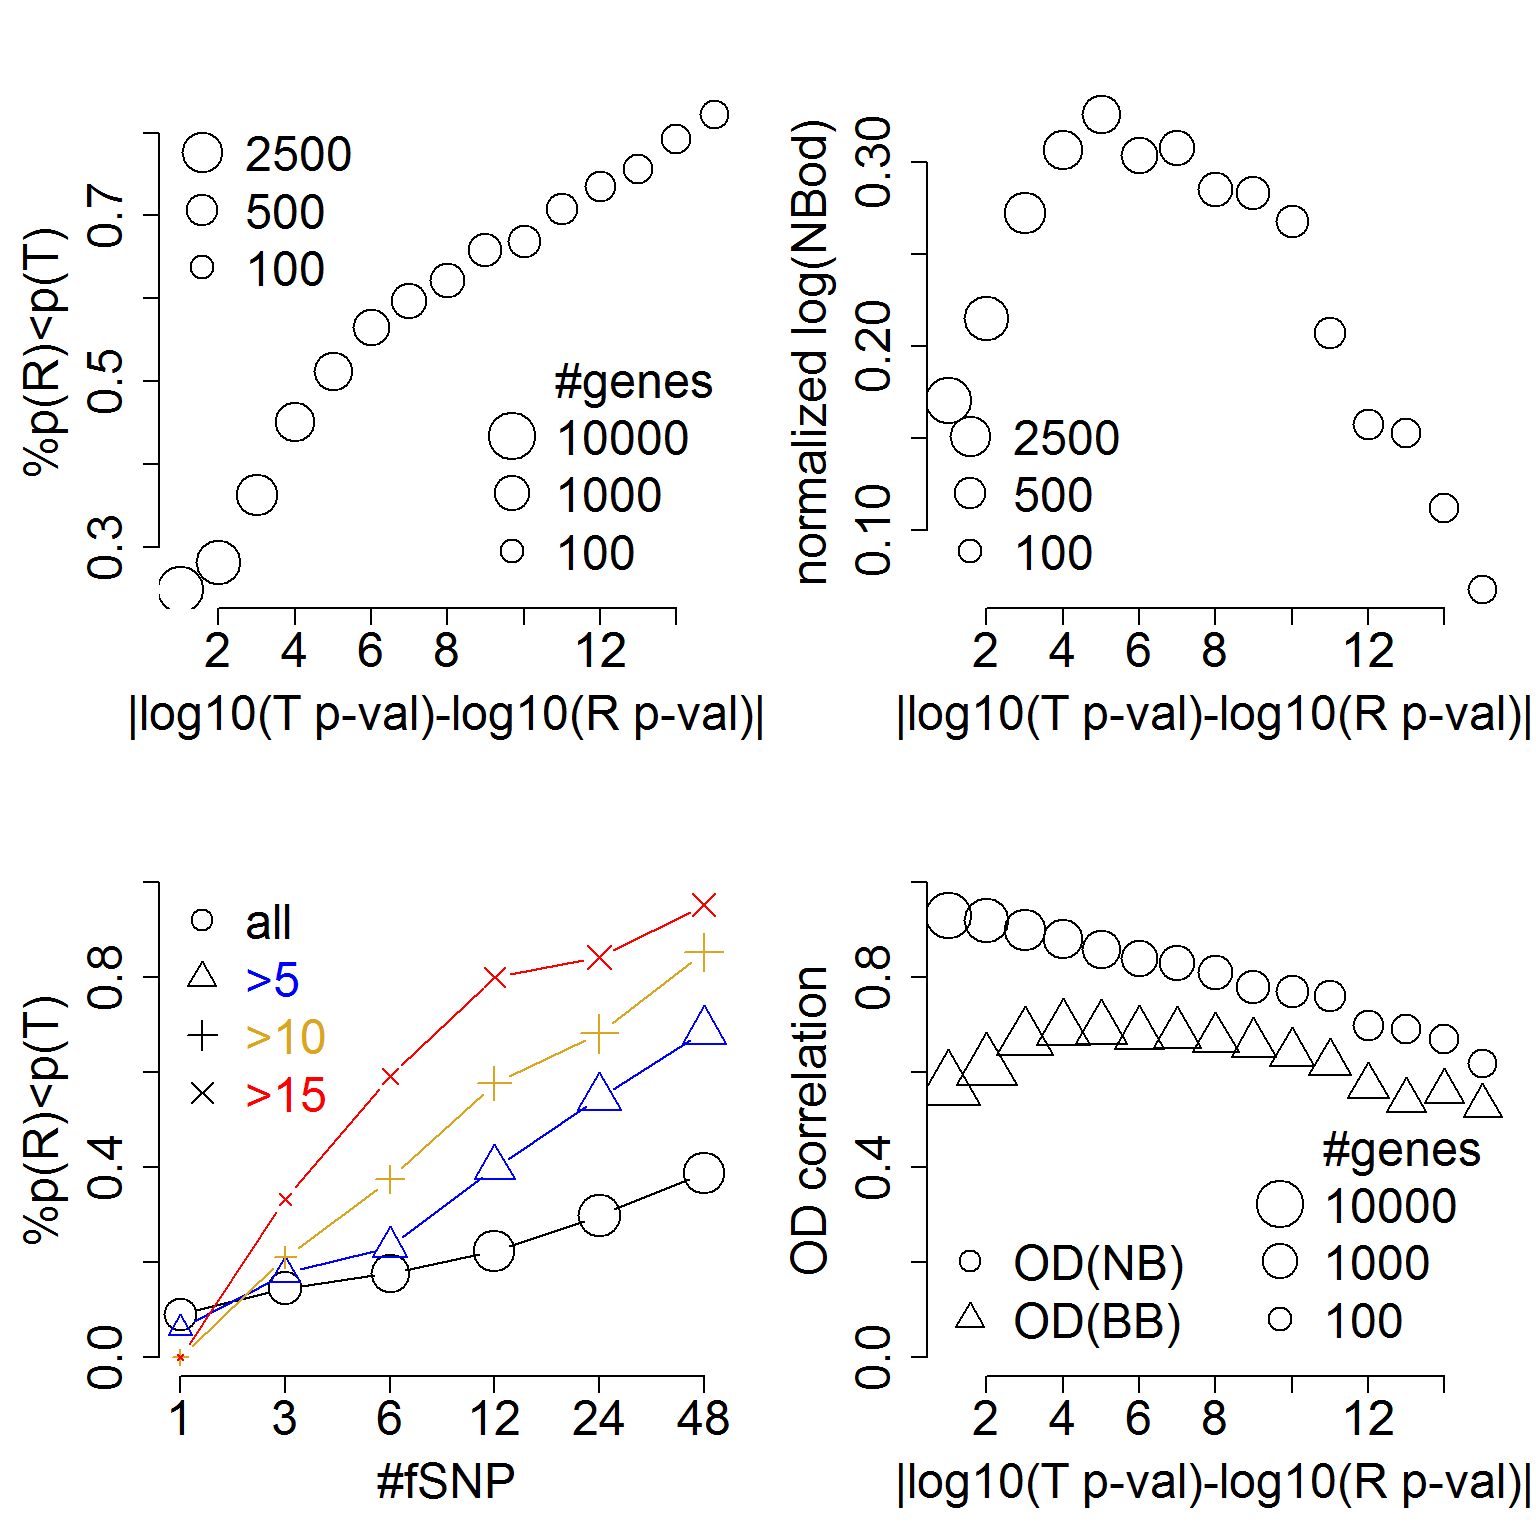
\includegraphics{markdown_files/figure-latex/fig1-1} \end{center}

Plotting Over-dispersions

\begin{Shaded}
\begin{Highlighting}[]
\KeywordTok{par}\NormalTok{(}\DataTypeTok{mfrow=}\KeywordTok{c}\NormalTok{(}\DecValTok{2}\NormalTok{,}\DecValTok{3}\NormalTok{))}
\KeywordTok{par}\NormalTok{(}\DataTypeTok{mar=}\KeywordTok{c}\NormalTok{(}\DecValTok{5}\NormalTok{,}\DecValTok{5}\NormalTok{,}\DecValTok{3}\NormalTok{,}\DecValTok{1}\NormalTok{))}

\KeywordTok{plot}\NormalTok{(}\KeywordTok{density}\NormalTok{(lodNB), }\DataTypeTok{bty=}\StringTok{"n"}\NormalTok{, }\DataTypeTok{main=}\StringTok{"log10(NB OD)"}\NormalTok{, }
     \DataTypeTok{xlab=}\StringTok{"log(od)"}\NormalTok{, }\DataTypeTok{cex.main=}\NormalTok{cexes, }\DataTypeTok{cex.lab=}\NormalTok{cexes, }\DataTypeTok{cex.axis=}\NormalTok{cexes)}
\KeywordTok{plot}\NormalTok{(}\KeywordTok{density}\NormalTok{(lodBB), }\DataTypeTok{bty=}\StringTok{"n"}\NormalTok{, }\DataTypeTok{main=}\StringTok{"log10(BB OD)"}\NormalTok{, }
     \DataTypeTok{xlab=}\StringTok{"log(od)"}\NormalTok{, }\DataTypeTok{cex.main=}\NormalTok{cexes, }\DataTypeTok{cex.lab=}\NormalTok{cexes, }\DataTypeTok{cex.axis=}\NormalTok{cexes)}
\KeywordTok{plot}\NormalTok{(}\KeywordTok{density}\NormalTok{(lodR), }\DataTypeTok{bty=}\StringTok{"n"}\NormalTok{, }\DataTypeTok{main=}\StringTok{"log10(RASQ OD)"}\NormalTok{,}
     \DataTypeTok{xlab=}\StringTok{"log(od)"}\NormalTok{, }\DataTypeTok{cex.main=}\NormalTok{cexes, }\DataTypeTok{cex.lab=}\NormalTok{cexes, }\DataTypeTok{cex.axis=}\NormalTok{cexes)}
\KeywordTok{plot}\NormalTok{(lodNB, lodBB, }\DataTypeTok{main=}\StringTok{"NB vs BB over-disp"}\NormalTok{, }\DataTypeTok{pch=}\DecValTok{20}\NormalTok{, }\DataTypeTok{cex=}\FloatTok{0.5}\NormalTok{, }\DataTypeTok{col=}\KeywordTok{rgb}\NormalTok{(}\FloatTok{0.8}\NormalTok{,}\FloatTok{0.1}\NormalTok{,}\FloatTok{0.1}\NormalTok{,}\FloatTok{0.5}\NormalTok{), }\DataTypeTok{bty=}\StringTok{"n"}\NormalTok{,}
     \DataTypeTok{xlab=}\StringTok{"log(NB OD)"}\NormalTok{, }\DataTypeTok{ylab=}\StringTok{"log(BB OD)"}\NormalTok{, }\DataTypeTok{cex.main=}\NormalTok{cexes, }\DataTypeTok{cex.lab=}\NormalTok{cexes, }\DataTypeTok{cex.axis=}\NormalTok{cexes)}
\KeywordTok{abline}\NormalTok{(}\DataTypeTok{a=}\DecValTok{0}\NormalTok{, }\DataTypeTok{b=}\DecValTok{1}\NormalTok{)}
\KeywordTok{plot}\NormalTok{(lodNB, lodR, }\DataTypeTok{main=}\StringTok{"NB vs Rasq over-disp"}\NormalTok{, }\DataTypeTok{pch=}\DecValTok{20}\NormalTok{, }\DataTypeTok{cex=}\FloatTok{0.5}\NormalTok{, }\DataTypeTok{col=}\KeywordTok{rgb}\NormalTok{(}\FloatTok{0.8}\NormalTok{,}\FloatTok{0.1}\NormalTok{,}\FloatTok{0.1}\NormalTok{,}\FloatTok{0.5}\NormalTok{), }\DataTypeTok{bty=}\StringTok{"n"}\NormalTok{,}
     \DataTypeTok{xlab=}\StringTok{"log(NB OD)"}\NormalTok{, }\DataTypeTok{ylab=}\StringTok{"log(RASQ OD)"}\NormalTok{, }\DataTypeTok{cex.main=}\NormalTok{cexes, }\DataTypeTok{cex.lab=}\NormalTok{cexes, }\DataTypeTok{cex.axis=}\NormalTok{cexes)}
\KeywordTok{abline}\NormalTok{(}\DataTypeTok{a=}\DecValTok{0}\NormalTok{, }\DataTypeTok{b=}\DecValTok{1}\NormalTok{)}
\KeywordTok{plot}\NormalTok{(lodR, lodBB, }\DataTypeTok{main=}\StringTok{"Rasq vs BB over-disp"}\NormalTok{, }\DataTypeTok{pch=}\DecValTok{20}\NormalTok{, }\DataTypeTok{cex=}\FloatTok{0.5}\NormalTok{, }\DataTypeTok{col=}\KeywordTok{rgb}\NormalTok{(}\FloatTok{0.8}\NormalTok{,}\FloatTok{0.1}\NormalTok{,}\FloatTok{0.1}\NormalTok{,}\FloatTok{0.5}\NormalTok{), }\DataTypeTok{bty=}\StringTok{"n"}\NormalTok{,}
     \DataTypeTok{xlab=}\StringTok{"log(RASQ OD)"}\NormalTok{, }\DataTypeTok{ylab=}\StringTok{"log(BB OD)"}\NormalTok{, }\DataTypeTok{cex.main=}\NormalTok{cexes, }\DataTypeTok{cex.lab=}\NormalTok{cexes, }\DataTypeTok{cex.axis=}\NormalTok{cexes)}
\KeywordTok{abline}\NormalTok{(}\DataTypeTok{a=}\DecValTok{0}\NormalTok{, }\DataTypeTok{b=}\DecValTok{1}\NormalTok{)}
\end{Highlighting}
\end{Shaded}

\begin{center}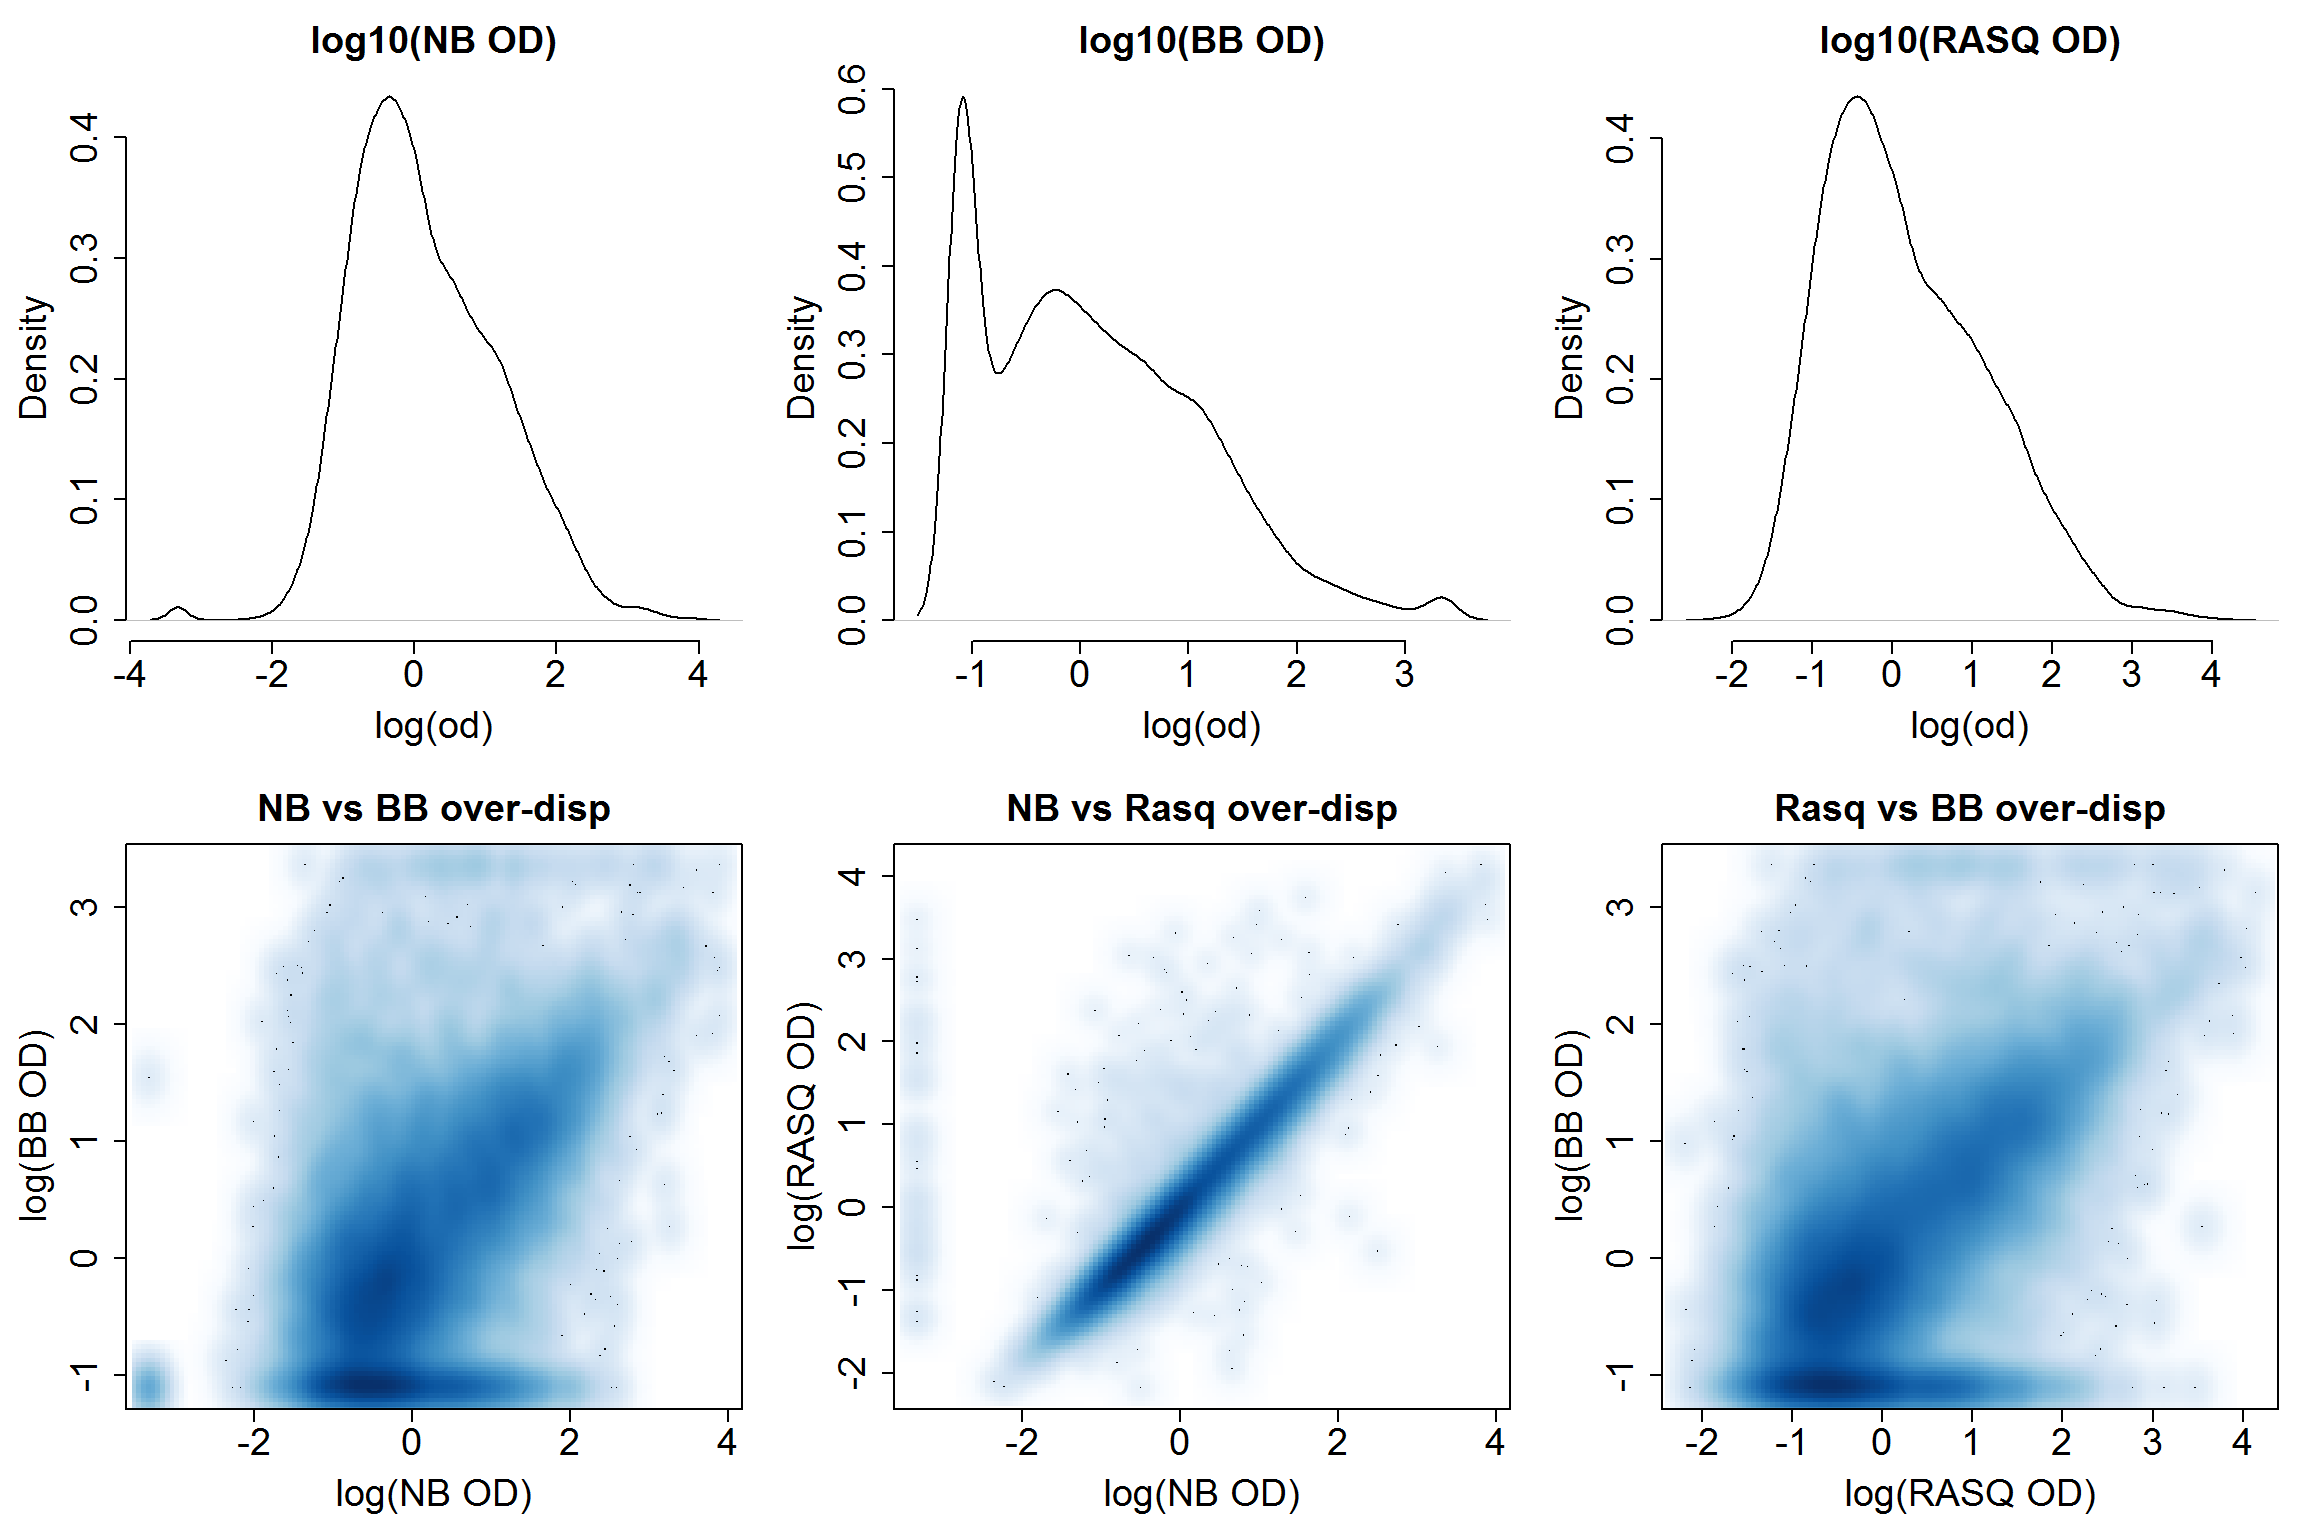
\includegraphics{markdown_files/figure-latex/fig2-1} \end{center}

Plotting RASQUAL read counts, normalized NfSNP and their interaction
along with interactions with BB over-dispersion

\begin{Shaded}
\begin{Highlighting}[]
\KeywordTok{par}\NormalTok{(}\DataTypeTok{mfrow=}\KeywordTok{c}\NormalTok{(}\DecValTok{2}\NormalTok{,}\DecValTok{3}\NormalTok{))}
\KeywordTok{par}\NormalTok{(}\DataTypeTok{mar=}\KeywordTok{c}\NormalTok{(}\DecValTok{5}\NormalTok{,}\DecValTok{5}\NormalTok{,}\DecValTok{3}\NormalTok{,}\DecValTok{1}\NormalTok{))}

\KeywordTok{plot}\NormalTok{(}\KeywordTok{density}\NormalTok{(asR), }\DataTypeTok{bty=}\StringTok{"n"}\NormalTok{, }\DataTypeTok{main=}\StringTok{"#as-RASQ"}\NormalTok{, }\DataTypeTok{xlab=}\StringTok{"#as-RASQUAL"}\NormalTok{, }\DataTypeTok{cex.main=}\NormalTok{cexes, }\DataTypeTok{cex.lab=}\NormalTok{cexes, }\DataTypeTok{cex.axis=}\NormalTok{cexes)}
\KeywordTok{plot}\NormalTok{(}\KeywordTok{density}\NormalTok{(NfSNP), }\DataTypeTok{bty=}\StringTok{"n"}\NormalTok{, }\DataTypeTok{main=}\StringTok{"#fSNPs"}\NormalTok{, }\DataTypeTok{xlab=}\StringTok{"#fSNPs"}\NormalTok{, }\DataTypeTok{cex.main=}\NormalTok{cexes, }\DataTypeTok{cex.lab=}\NormalTok{cexes, }\DataTypeTok{cex.axis=}\NormalTok{cexes)}
\CommentTok{#plot(density(NrSNP), bty="n", main="#rSNPs", xlab="#fSNPs", cex.main=cexes, cex.lab=cexes, cex.axis=cexes)}
\KeywordTok{plot}\NormalTok{(}\KeywordTok{density}\NormalTok{(i12), }\DataTypeTok{bty=}\StringTok{"n"}\NormalTok{, }\DataTypeTok{main=}\StringTok{"interac, #asR & #fSNP"}\NormalTok{, }
     \DataTypeTok{xlab=}\StringTok{"#as-RASQ * #fSNPs"}\NormalTok{, }\DataTypeTok{cex.main=}\NormalTok{cexes, }\DataTypeTok{cex.lab=}\NormalTok{cexes, }\DataTypeTok{cex.axis=}\NormalTok{cexes)}
\KeywordTok{plot}\NormalTok{(}\KeywordTok{density}\NormalTok{(i13), }\DataTypeTok{bty=}\StringTok{"n"}\NormalTok{, }\DataTypeTok{main=}\StringTok{"interac, #asR & #log(BB OD)"}\NormalTok{, }
     \DataTypeTok{xlab=}\StringTok{"#asR * log10(BB OD)"}\NormalTok{, }\DataTypeTok{cex.main=}\NormalTok{cexes, }\DataTypeTok{cex.lab=}\NormalTok{cexes, }\DataTypeTok{cex.axis=}\NormalTok{cexes)}
\KeywordTok{plot}\NormalTok{(}\KeywordTok{density}\NormalTok{(i23), }\DataTypeTok{bty=}\StringTok{"n"}\NormalTok{, }\DataTypeTok{main=}\StringTok{"interac, #fSNP & log(BB OD)"}\NormalTok{, }
     \DataTypeTok{xlab=}\StringTok{"#fSNPs * log10(BB OD)"}\NormalTok{, }\DataTypeTok{cex.main=}\NormalTok{cexes, }\DataTypeTok{cex.lab=}\NormalTok{cexes, }\DataTypeTok{cex.axis=}\NormalTok{cexes)}
\KeywordTok{plot}\NormalTok{(}\KeywordTok{density}\NormalTok{(i123), }\DataTypeTok{bty=}\StringTok{"n"}\NormalTok{, }\DataTypeTok{main=}\StringTok{"interac, #asR & #fSNP & log(BB OD0"}\NormalTok{, }\DataTypeTok{xlim=}\KeywordTok{c}\NormalTok{(}\OperatorTok{-}\DecValTok{10}\NormalTok{,}\DecValTok{10}\NormalTok{),}
     \DataTypeTok{xlab=}\StringTok{"#as-RASQ * #fSNPs * log10(BB OD)"}\NormalTok{, , }\DataTypeTok{cex.main=}\NormalTok{cexes, }\DataTypeTok{cex.lab=}\NormalTok{cexes, }\DataTypeTok{cex.axis=}\NormalTok{cexes)}
\end{Highlighting}
\end{Shaded}

\begin{center}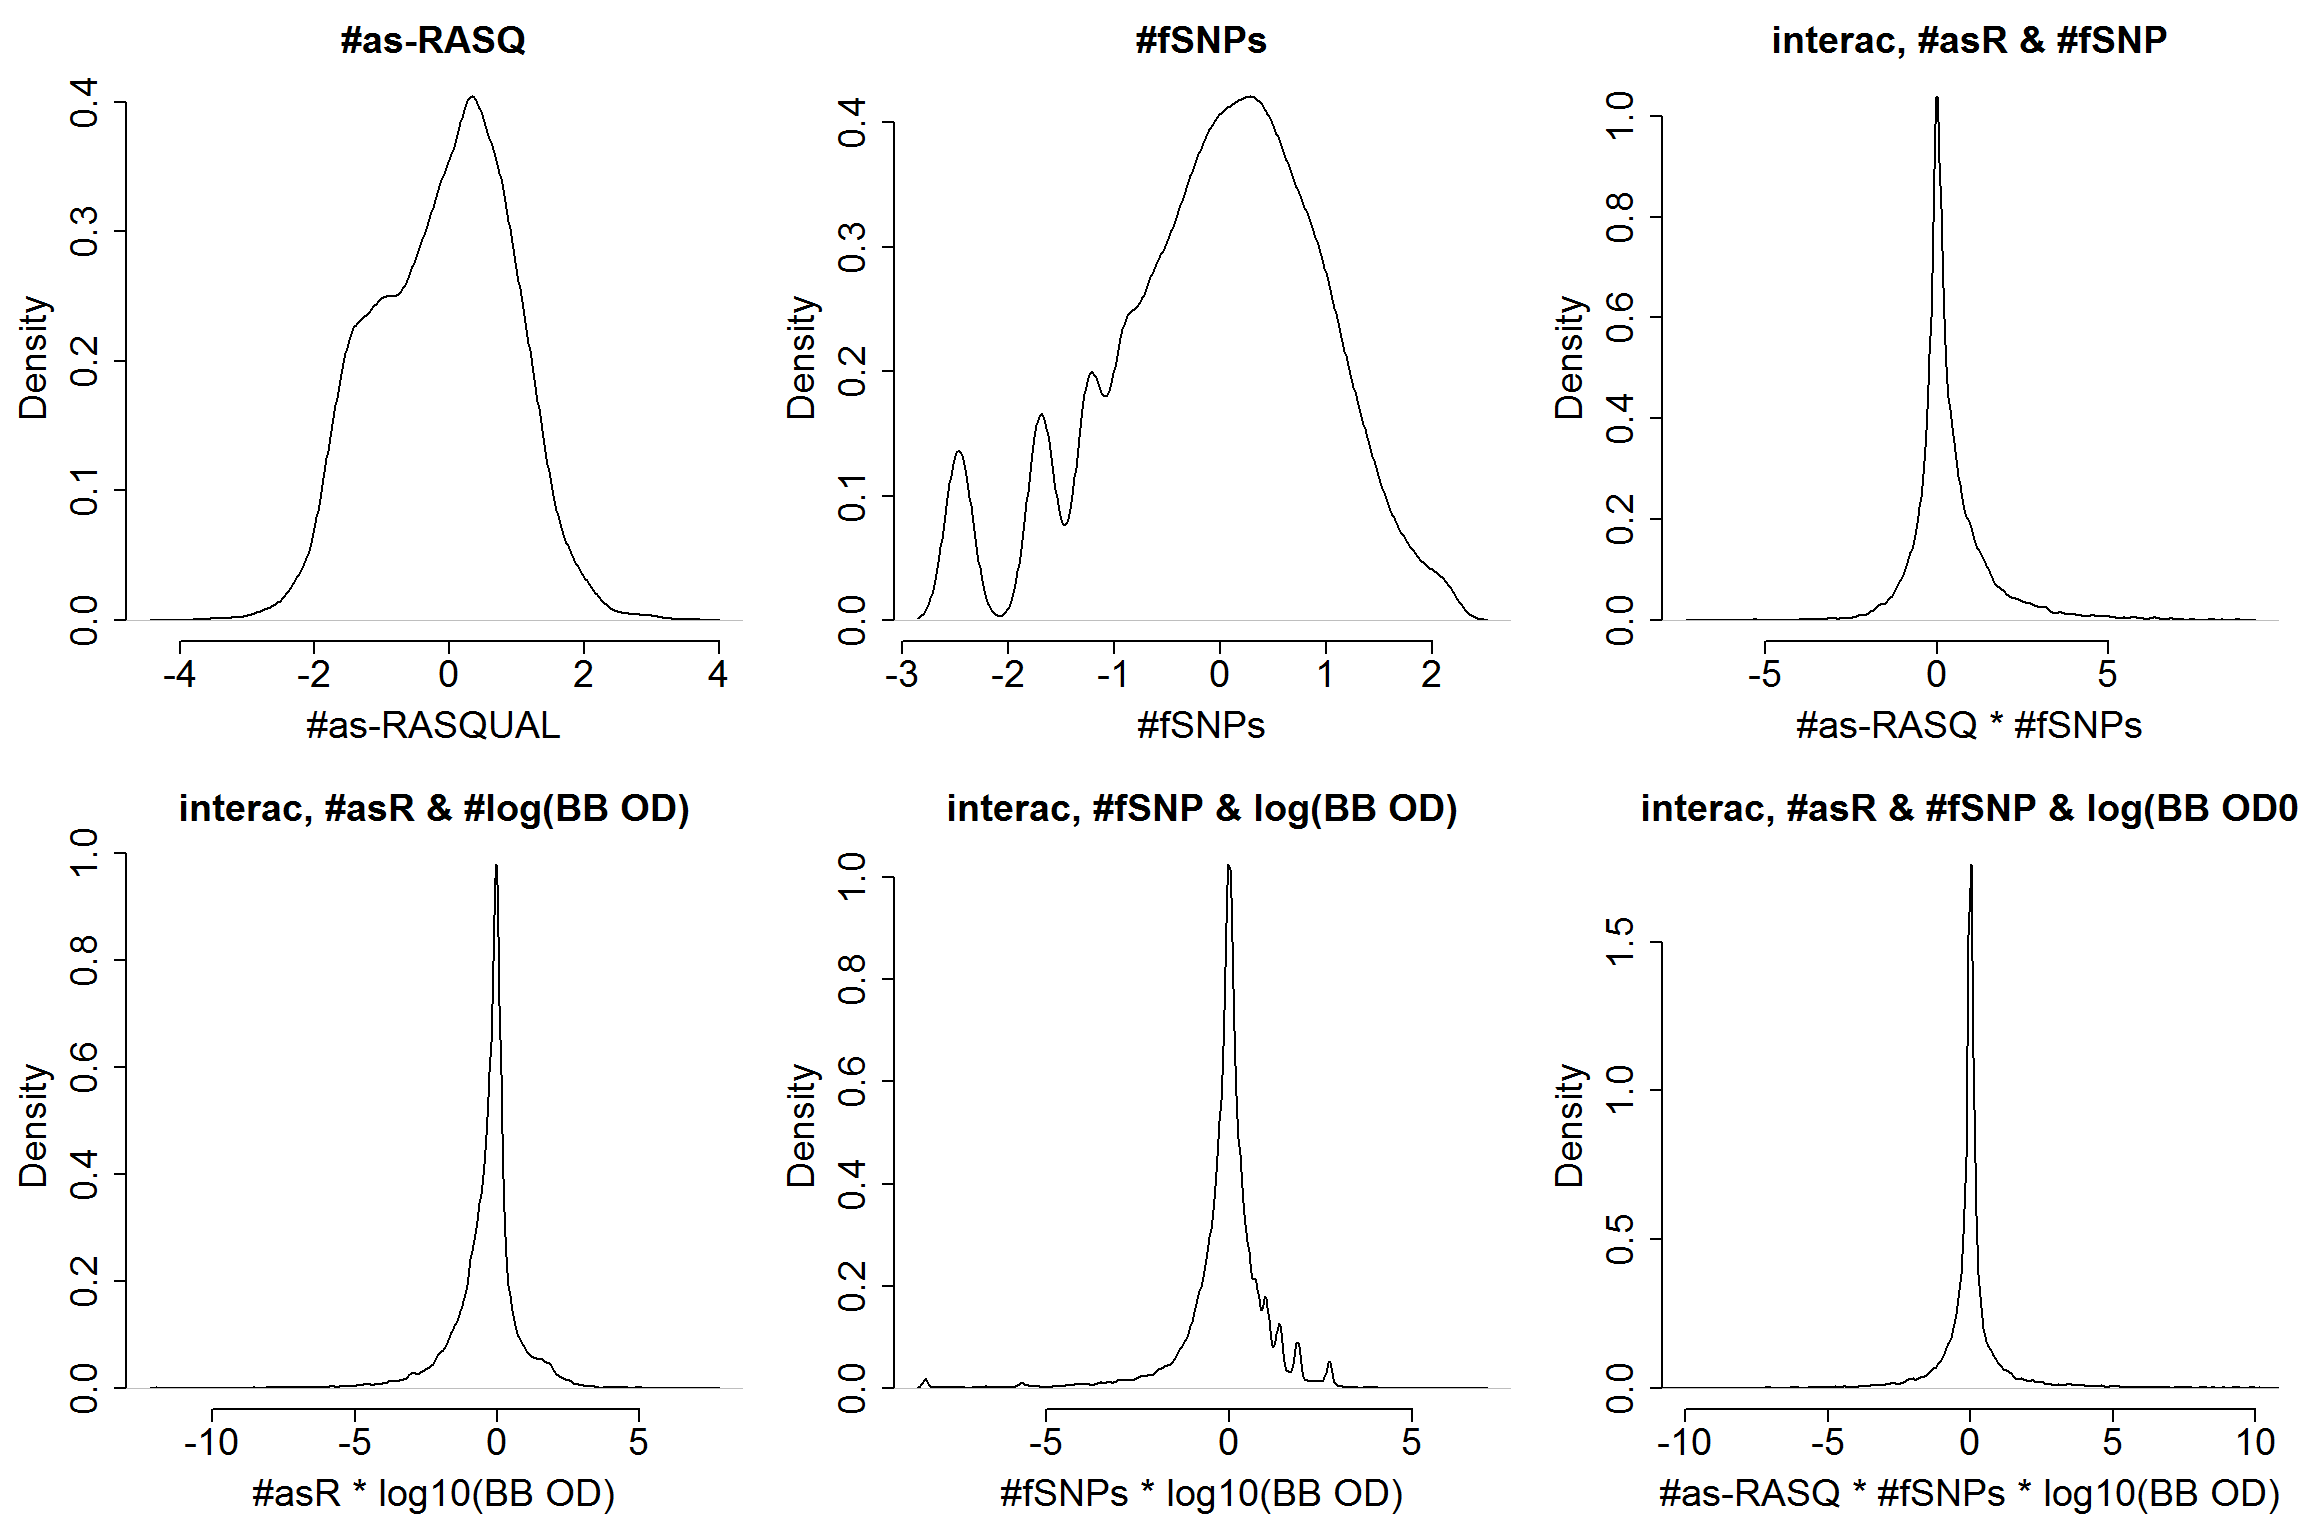
\includegraphics{markdown_files/figure-latex/fig3-1} \end{center}

\begin{Shaded}
\begin{Highlighting}[]
\KeywordTok{par}\NormalTok{(}\DataTypeTok{mfrow=}\KeywordTok{c}\NormalTok{(}\DecValTok{2}\NormalTok{,}\DecValTok{3}\NormalTok{))}
\KeywordTok{par}\NormalTok{(}\DataTypeTok{mar=}\KeywordTok{c}\NormalTok{(}\DecValTok{5}\NormalTok{,}\DecValTok{5}\NormalTok{,}\DecValTok{3}\NormalTok{,}\DecValTok{1}\NormalTok{))}

\KeywordTok{plot}\NormalTok{(}\KeywordTok{density}\NormalTok{(asT), }\DataTypeTok{bty=}\StringTok{"n"}\NormalTok{, }\DataTypeTok{main=}\StringTok{"#as-TReCASE"}\NormalTok{, }
     \DataTypeTok{xlab=}\StringTok{"#as-TReCASE"}\NormalTok{, }\DataTypeTok{cex.main=}\NormalTok{cexes, }\DataTypeTok{cex.lab=}\NormalTok{cexes, }\DataTypeTok{cex.axis=}\NormalTok{cexes)}
\KeywordTok{plot}\NormalTok{(}\KeywordTok{density}\NormalTok{(ia14), }\DataTypeTok{bty=}\StringTok{"n"}\NormalTok{, }\DataTypeTok{main=}\StringTok{"interact, #as-RASQ & #as-TReCASE"}\NormalTok{, }
     \DataTypeTok{xlab=}\StringTok{"#as-RASQ*#as-TReCASE"}\NormalTok{, }\DataTypeTok{cex.main=}\NormalTok{cexes, }\DataTypeTok{cex.lab=}\NormalTok{cexes, }\DataTypeTok{cex.axis=}\NormalTok{cexes)}
\KeywordTok{plot}\NormalTok{(asT, asR, }\DataTypeTok{bty=}\StringTok{"n"}\NormalTok{, }\DataTypeTok{main=}\StringTok{"#as-RASQ vs #as-TReCASE"}\NormalTok{, }\DataTypeTok{pch=}\DecValTok{20}\NormalTok{, }\DataTypeTok{cex=}\FloatTok{0.5}\NormalTok{, }\DataTypeTok{col=}\KeywordTok{rgb}\NormalTok{(}\FloatTok{0.8}\NormalTok{,}\FloatTok{0.1}\NormalTok{,}\FloatTok{0.1}\NormalTok{,}\FloatTok{0.5}\NormalTok{), }\DataTypeTok{bty=}\StringTok{"n"}\NormalTok{, }
              \DataTypeTok{xlab=}\StringTok{"#as-TReCASE"}\NormalTok{, }\DataTypeTok{ylab=}\StringTok{"#as-RASQUAL"}\NormalTok{, }\DataTypeTok{cex.main=}\NormalTok{cexes, }\DataTypeTok{cex.lab=}\NormalTok{cexes, }\DataTypeTok{cex.axis=}\NormalTok{cexes)}

\KeywordTok{plot}\NormalTok{(}\KeywordTok{density}\NormalTok{(NrSNP), }\DataTypeTok{bty=}\StringTok{"n"}\NormalTok{, }\DataTypeTok{main=}\StringTok{"#rSNPs"}\NormalTok{, }
     \DataTypeTok{xlab=}\StringTok{"#fSNPs"}\NormalTok{, }\DataTypeTok{cex.main=}\NormalTok{cexes, }\DataTypeTok{cex.lab=}\NormalTok{cexes, }\DataTypeTok{cex.axis=}\NormalTok{cexes)}
\KeywordTok{plot}\NormalTok{(}\KeywordTok{density}\NormalTok{(y), }\DataTypeTok{bty=}\StringTok{"n"}\NormalTok{, }\DataTypeTok{main=}\StringTok{"difference in log10 p-values"}\NormalTok{, }
     \DataTypeTok{xlab=}\StringTok{"log10(T p-val)-log10(R p-val)"}\NormalTok{, }\DataTypeTok{cex.main=}\NormalTok{cexes, }\DataTypeTok{cex.lab=}\NormalTok{cexes, }\DataTypeTok{cex.axis=}\NormalTok{cexes)}
\KeywordTok{plot}\NormalTok{(rasq}\OperatorTok{$}\NormalTok{tnlt, rasq}\OperatorTok{$}\NormalTok{rnlt, }\DataTypeTok{bty=}\StringTok{"n"}\NormalTok{, }\DataTypeTok{main=}\StringTok{"RASQUAL vs TReCASE p-val"}\NormalTok{, }\DataTypeTok{pch=}\DecValTok{20}\NormalTok{, }\DataTypeTok{cex=}\FloatTok{0.5}\NormalTok{, }\DataTypeTok{col=}\KeywordTok{rgb}\NormalTok{(}\FloatTok{0.8}\NormalTok{,}\FloatTok{0.1}\NormalTok{,}\FloatTok{0.1}\NormalTok{,}\FloatTok{0.5}\NormalTok{), }\DataTypeTok{bty=}\StringTok{"n"}\NormalTok{, }
              \DataTypeTok{xlab=}\StringTok{"-log10(T p-val)"}\NormalTok{, }\DataTypeTok{ylab=}\StringTok{"-log10(R p-val)"}\NormalTok{, }\DataTypeTok{cex.main=}\NormalTok{cexes, }\DataTypeTok{cex.lab=}\NormalTok{cexes, }\DataTypeTok{cex.axis=}\NormalTok{cexes)}
\end{Highlighting}
\end{Shaded}

\begin{center}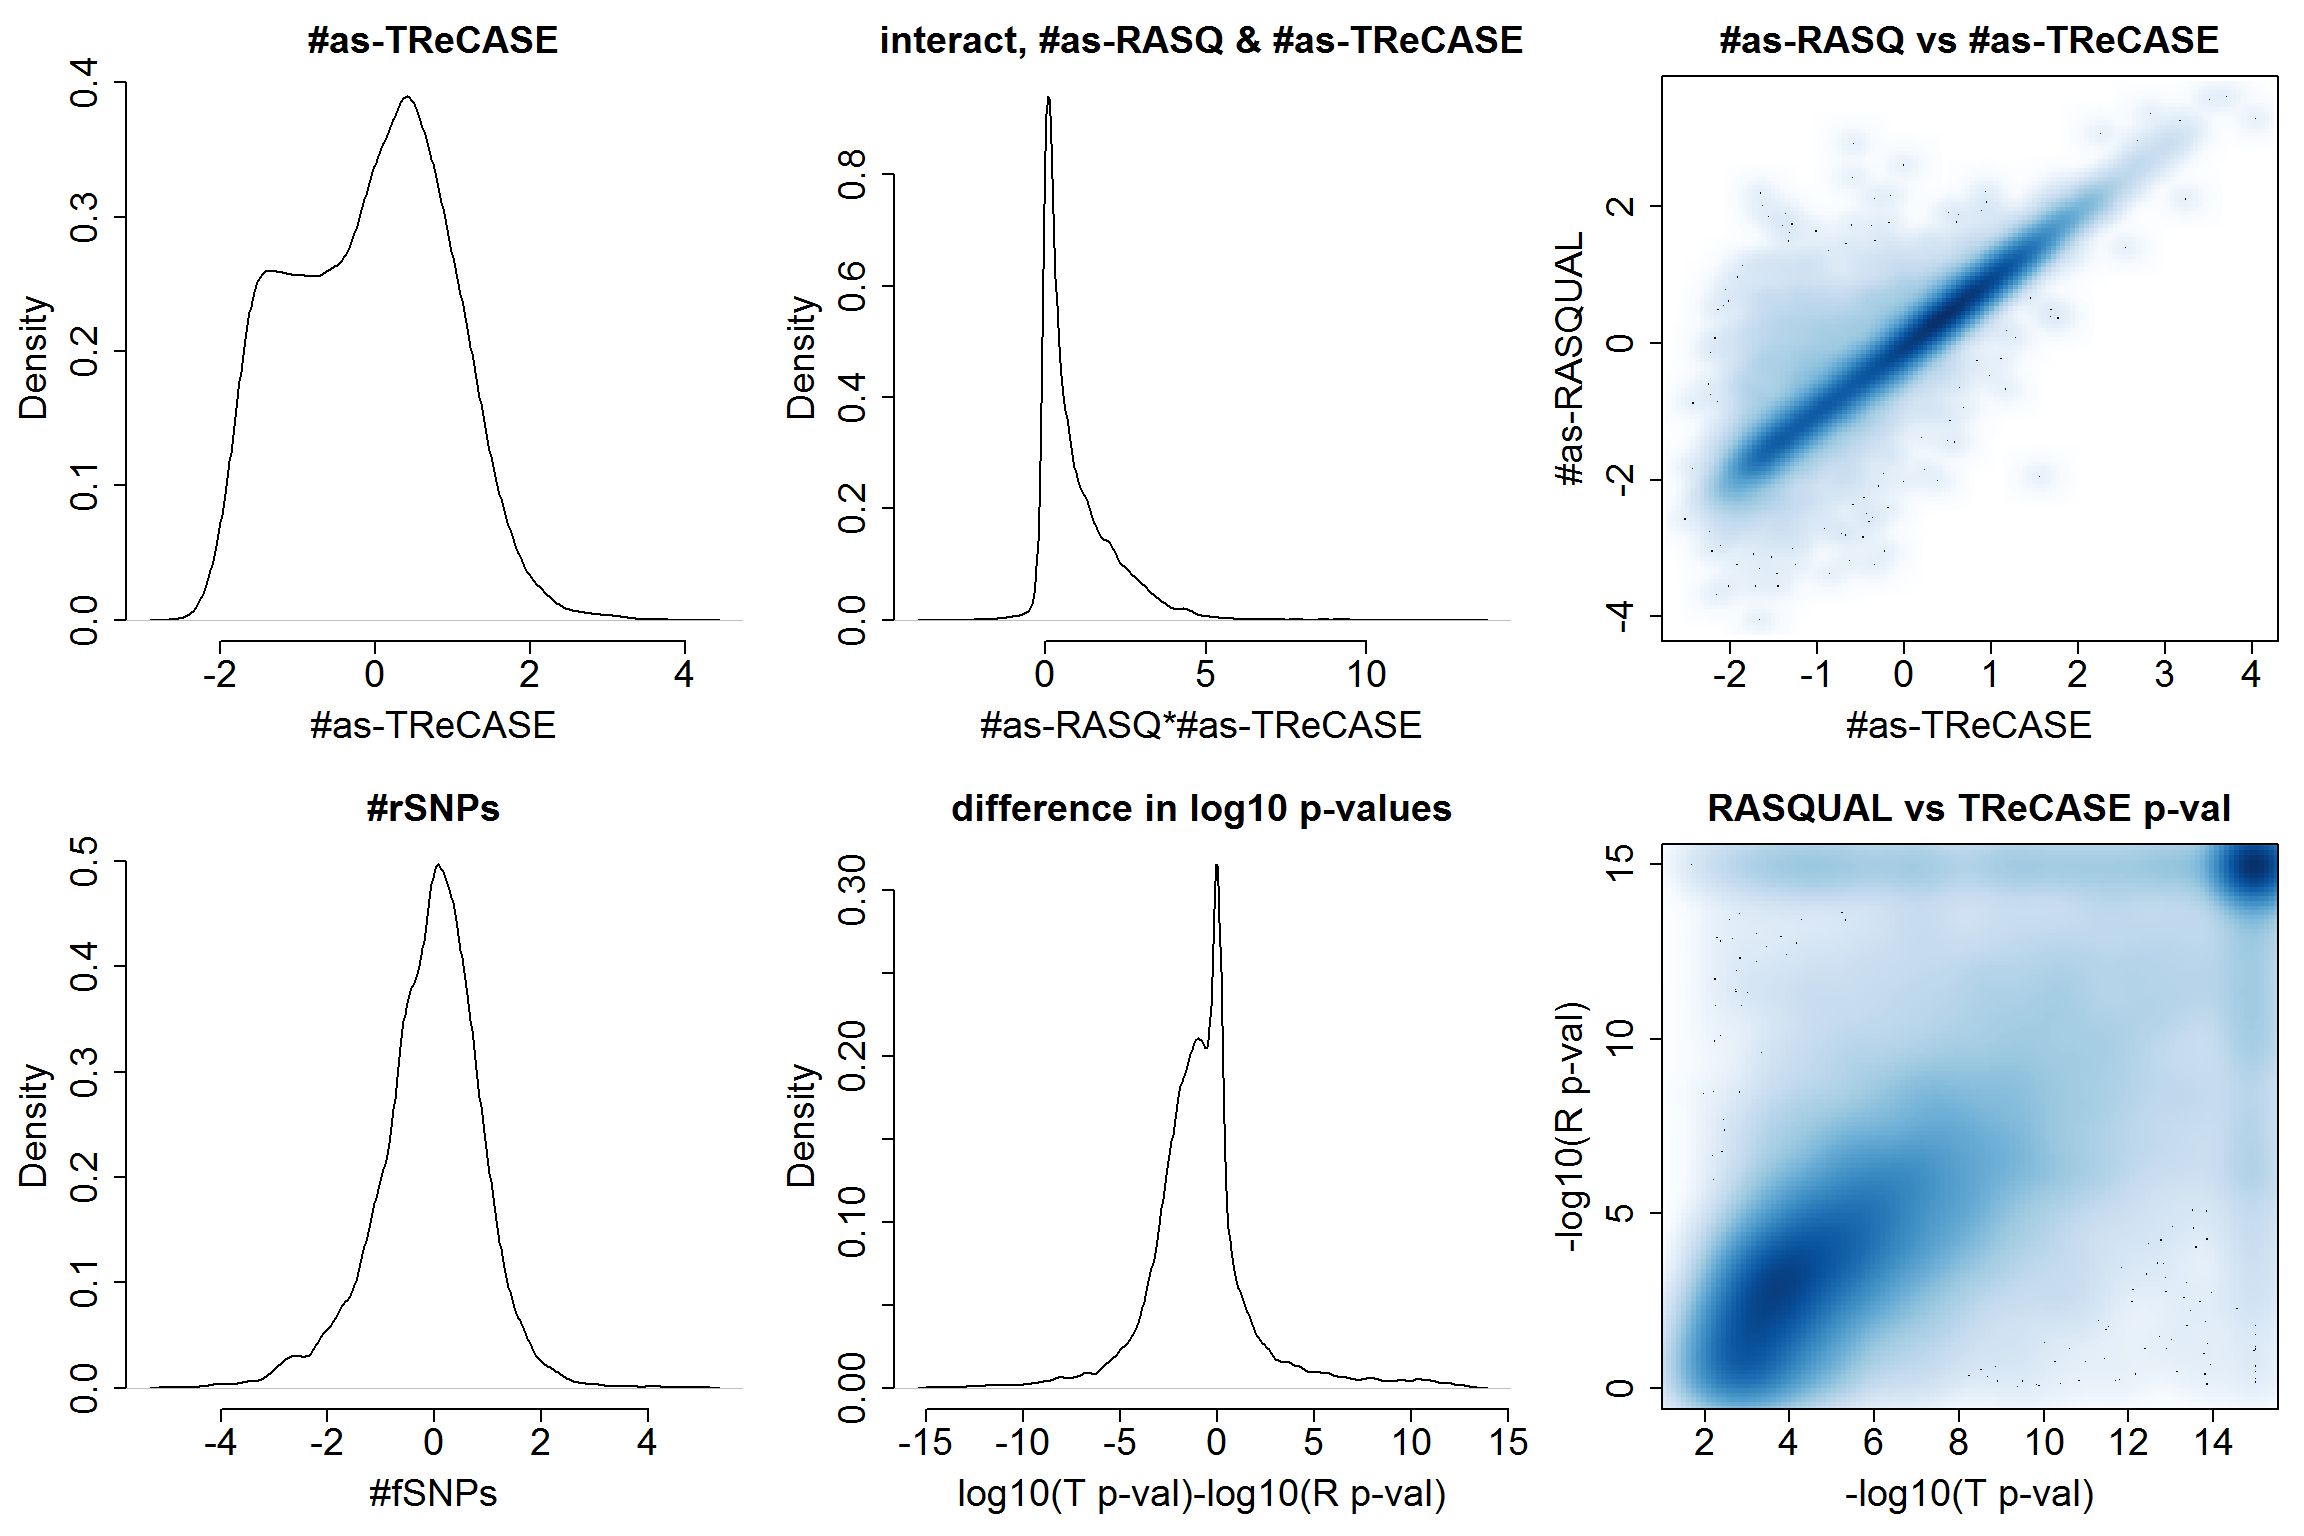
\includegraphics{markdown_files/figure-latex/fig4-1} \end{center}

\begin{Shaded}
\begin{Highlighting}[]
\CommentTok{#rasq$rnlt-rasq$tnlt") - negative implies TReCASE is more significant}
\end{Highlighting}
\end{Shaded}

Other covariates: median permuted p-value, mapping error, reference bias
and Chi2 of Hardy Weinberg Equilibrium

\begin{Shaded}
\begin{Highlighting}[]
\KeywordTok{par}\NormalTok{(}\DataTypeTok{mfrow=}\KeywordTok{c}\NormalTok{(}\DecValTok{2}\NormalTok{,}\DecValTok{2}\NormalTok{))}
\KeywordTok{par}\NormalTok{(}\DataTypeTok{mar=}\KeywordTok{c}\NormalTok{(}\DecValTok{5}\NormalTok{,}\DecValTok{5}\NormalTok{,}\DecValTok{3}\NormalTok{,}\DecValTok{1}\NormalTok{))}
\KeywordTok{plot}\NormalTok{(}\KeywordTok{density}\NormalTok{(mpp), }\DataTypeTok{bty=}\StringTok{"n"}\NormalTok{, }\DataTypeTok{main=}\StringTok{"#median permuted p-val"}\NormalTok{, }
     \DataTypeTok{xlab=}\StringTok{"normalized p-value"}\NormalTok{, }\DataTypeTok{cex.main=}\NormalTok{cexes, }\DataTypeTok{cex.lab=}\NormalTok{cexes, }\DataTypeTok{cex.axis=}\NormalTok{cexes)}
\KeywordTok{plot}\NormalTok{(}\KeywordTok{density}\NormalTok{(derr), }\DataTypeTok{bty=}\StringTok{"n"}\NormalTok{, }\DataTypeTok{main=}\StringTok{"mapping error"}\NormalTok{, }
     \DataTypeTok{xlab=}\StringTok{"normalized error"}\NormalTok{, }\DataTypeTok{cex.main=}\NormalTok{cexes, }\DataTypeTok{cex.lab=}\NormalTok{cexes, }\DataTypeTok{cex.axis=}\NormalTok{cexes)}
\KeywordTok{plot}\NormalTok{(}\KeywordTok{density}\NormalTok{(phib), }\DataTypeTok{bty=}\StringTok{"n"}\NormalTok{, }\DataTypeTok{main=}\StringTok{"#reference bias"}\NormalTok{, }
     \DataTypeTok{xlab=}\StringTok{"normalized deviation from 0.5"}\NormalTok{, }\DataTypeTok{cex.main=}\NormalTok{cexes, }\DataTypeTok{cex.lab=}\NormalTok{cexes, }\DataTypeTok{cex.axis=}\NormalTok{cexes)}
\KeywordTok{plot}\NormalTok{(}\KeywordTok{density}\NormalTok{(hwec2), }\DataTypeTok{bty=}\StringTok{"n"}\NormalTok{, }\DataTypeTok{main=}\StringTok{"#HWE equilibrium"}\NormalTok{, }
     \DataTypeTok{xlab=}\StringTok{"log(Chi2)"}\NormalTok{, }\DataTypeTok{cex.main=}\NormalTok{cexes, }\DataTypeTok{cex.lab=}\NormalTok{cexes, }\DataTypeTok{cex.axis=}\NormalTok{cexes)}
\end{Highlighting}
\end{Shaded}

\begin{center}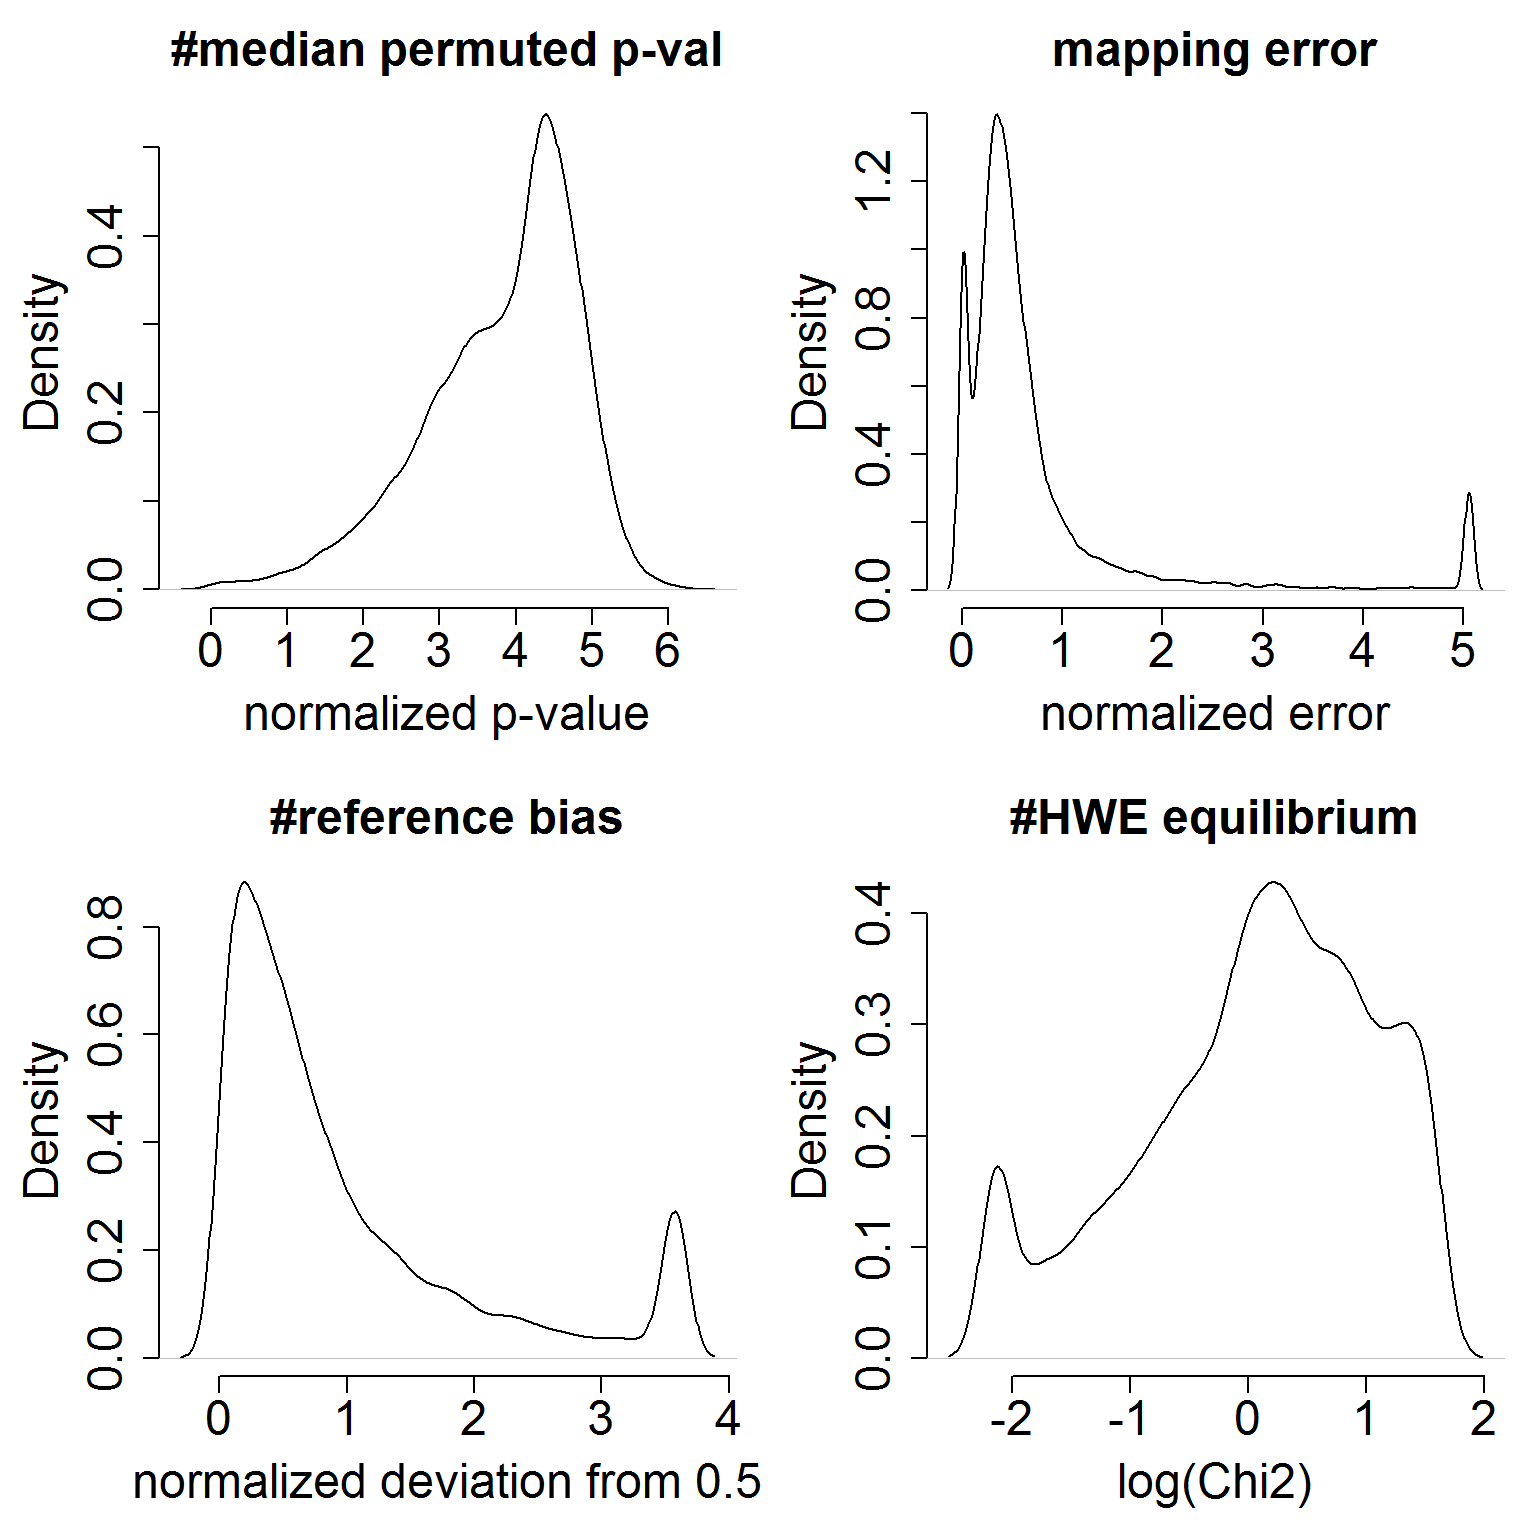
\includegraphics{markdown_files/figure-latex/fig5-1} \end{center}

Plotting RASQUAL read counts, normalized NfSNP and their interaction
along with interactions with BB over-dispersion

\begin{Shaded}
\begin{Highlighting}[]
\KeywordTok{par}\NormalTok{(}\DataTypeTok{mfrow=}\KeywordTok{c}\NormalTok{(}\DecValTok{2}\NormalTok{,}\DecValTok{3}\NormalTok{))}
\KeywordTok{par}\NormalTok{(}\DataTypeTok{mar=}\KeywordTok{c}\NormalTok{(}\DecValTok{5}\NormalTok{,}\DecValTok{5}\NormalTok{,}\DecValTok{3}\NormalTok{,}\DecValTok{1}\NormalTok{))}

\KeywordTok{plot}\NormalTok{(lodNB, y, }\DataTypeTok{main=}\StringTok{"discrep. vs log(NB)"}\NormalTok{, }\DataTypeTok{ylab=}\StringTok{"diff"}\NormalTok{, }\DataTypeTok{pch=}\DecValTok{20}\NormalTok{, }\DataTypeTok{cex=}\FloatTok{0.5}\NormalTok{, }\DataTypeTok{col=}\KeywordTok{rgb}\NormalTok{(}\FloatTok{0.8}\NormalTok{,}\FloatTok{0.1}\NormalTok{,}\FloatTok{0.1}\NormalTok{,}\FloatTok{0.5}\NormalTok{), }
     \DataTypeTok{xlab=}\StringTok{"log(NB OD)"}\NormalTok{, }\DataTypeTok{cex.main=}\NormalTok{cexes,  }\DataTypeTok{cex.lab=}\NormalTok{cexes, }\DataTypeTok{cex.axis=}\NormalTok{cexes, }\DataTypeTok{bty=}\StringTok{"n"}\NormalTok{)}
\KeywordTok{plot}\NormalTok{(lodBB, y, }\DataTypeTok{main=}\StringTok{"discrep. vs log(BB)"}\NormalTok{, }\DataTypeTok{ylab=}\StringTok{"diff"}\NormalTok{, }\DataTypeTok{pch=}\DecValTok{20}\NormalTok{, }\DataTypeTok{cex=}\FloatTok{0.5}\NormalTok{, }\DataTypeTok{col=}\KeywordTok{rgb}\NormalTok{(}\FloatTok{0.8}\NormalTok{,}\FloatTok{0.1}\NormalTok{,}\FloatTok{0.1}\NormalTok{,}\FloatTok{0.5}\NormalTok{),  }
     \DataTypeTok{xlab=}\StringTok{"log(BB OD)"}\NormalTok{, }\DataTypeTok{cex.main=}\NormalTok{cexes, }\DataTypeTok{cex.lab=}\NormalTok{cexes, }\DataTypeTok{cex.axis=}\NormalTok{cexes, }\DataTypeTok{bty=}\StringTok{"n"}\NormalTok{)}
\KeywordTok{plot}\NormalTok{(NfSNP, y, }\DataTypeTok{main=}\StringTok{"discrep. vs #fSNP"}\NormalTok{, }\DataTypeTok{ylab=}\StringTok{"diff"}\NormalTok{, }\DataTypeTok{pch=}\DecValTok{20}\NormalTok{, }\DataTypeTok{cex=}\FloatTok{0.5}\NormalTok{, }\DataTypeTok{col=}\KeywordTok{rgb}\NormalTok{(}\FloatTok{0.8}\NormalTok{,}\FloatTok{0.1}\NormalTok{,}\FloatTok{0.1}\NormalTok{,}\FloatTok{0.5}\NormalTok{), }
     \DataTypeTok{xlab=}\StringTok{"num-fSNP"}\NormalTok{, }\DataTypeTok{cex.main=}\NormalTok{cexes, }\DataTypeTok{cex.lab=}\NormalTok{cexes, }\DataTypeTok{cex.axis=}\NormalTok{cexes, }\DataTypeTok{bty=}\StringTok{"n"}\NormalTok{)}
\KeywordTok{plot}\NormalTok{(asR, y, }\DataTypeTok{main=}\StringTok{"discrep. vs ASReC-RL cnt"}\NormalTok{, }\DataTypeTok{ylab=}\StringTok{"diff"}\NormalTok{,  }\DataTypeTok{pch=}\DecValTok{20}\NormalTok{, }\DataTypeTok{cex=}\FloatTok{0.5}\NormalTok{, }\DataTypeTok{col=}\KeywordTok{rgb}\NormalTok{(}\FloatTok{0.8}\NormalTok{,}\FloatTok{0.1}\NormalTok{,}\FloatTok{0.1}\NormalTok{,}\FloatTok{0.5}\NormalTok{),}
     \DataTypeTok{xlab=}\StringTok{"ASReC-RL"}\NormalTok{, }\DataTypeTok{cex.main=}\NormalTok{cexes, }\DataTypeTok{cex.lab=}\NormalTok{cexes,}\DataTypeTok{cex.axis=}\NormalTok{cexes, }\DataTypeTok{bty=}\StringTok{"n"}\NormalTok{)}
\KeywordTok{plot}\NormalTok{(asT, y, }\DataTypeTok{main=}\StringTok{"discrep. vs ASReC-TR cnt"}\NormalTok{, }\DataTypeTok{ylab=}\StringTok{"diff"}\NormalTok{,  }\DataTypeTok{pch=}\DecValTok{20}\NormalTok{, }\DataTypeTok{cex=}\FloatTok{0.5}\NormalTok{, }\DataTypeTok{col=}\KeywordTok{rgb}\NormalTok{(}\FloatTok{0.8}\NormalTok{,}\FloatTok{0.1}\NormalTok{,}\FloatTok{0.1}\NormalTok{,}\FloatTok{0.5}\NormalTok{),}
     \DataTypeTok{xlab=}\StringTok{"ASReC-TR"}\NormalTok{, }\DataTypeTok{cex.main=}\NormalTok{cexes, }\DataTypeTok{cex.lab=}\NormalTok{cexes, }\DataTypeTok{cex.axis=}\NormalTok{cexes, }\DataTypeTok{bty=}\StringTok{"n"}\NormalTok{)}
\KeywordTok{plot}\NormalTok{(mpp, y, }\DataTypeTok{main=}\StringTok{"discrep. vs med. per. p-val"}\NormalTok{, }\DataTypeTok{ylab=}\StringTok{"diff"}\NormalTok{,  }\DataTypeTok{pch=}\DecValTok{20}\NormalTok{, }\DataTypeTok{cex=}\FloatTok{0.5}\NormalTok{, }\DataTypeTok{col=}\KeywordTok{rgb}\NormalTok{(}\FloatTok{0.8}\NormalTok{,}\FloatTok{0.1}\NormalTok{,}\FloatTok{0.1}\NormalTok{,}\FloatTok{0.5}\NormalTok{), }
     \DataTypeTok{xlab=}\StringTok{"med. per. p-val"}\NormalTok{, }\DataTypeTok{cex.main=}\NormalTok{cexes, }\DataTypeTok{cex.lab=}\NormalTok{cexes, }\DataTypeTok{cex.axis=}\NormalTok{cexes, }\DataTypeTok{bty=}\StringTok{"n"}\NormalTok{)}
\end{Highlighting}
\end{Shaded}

\begin{center}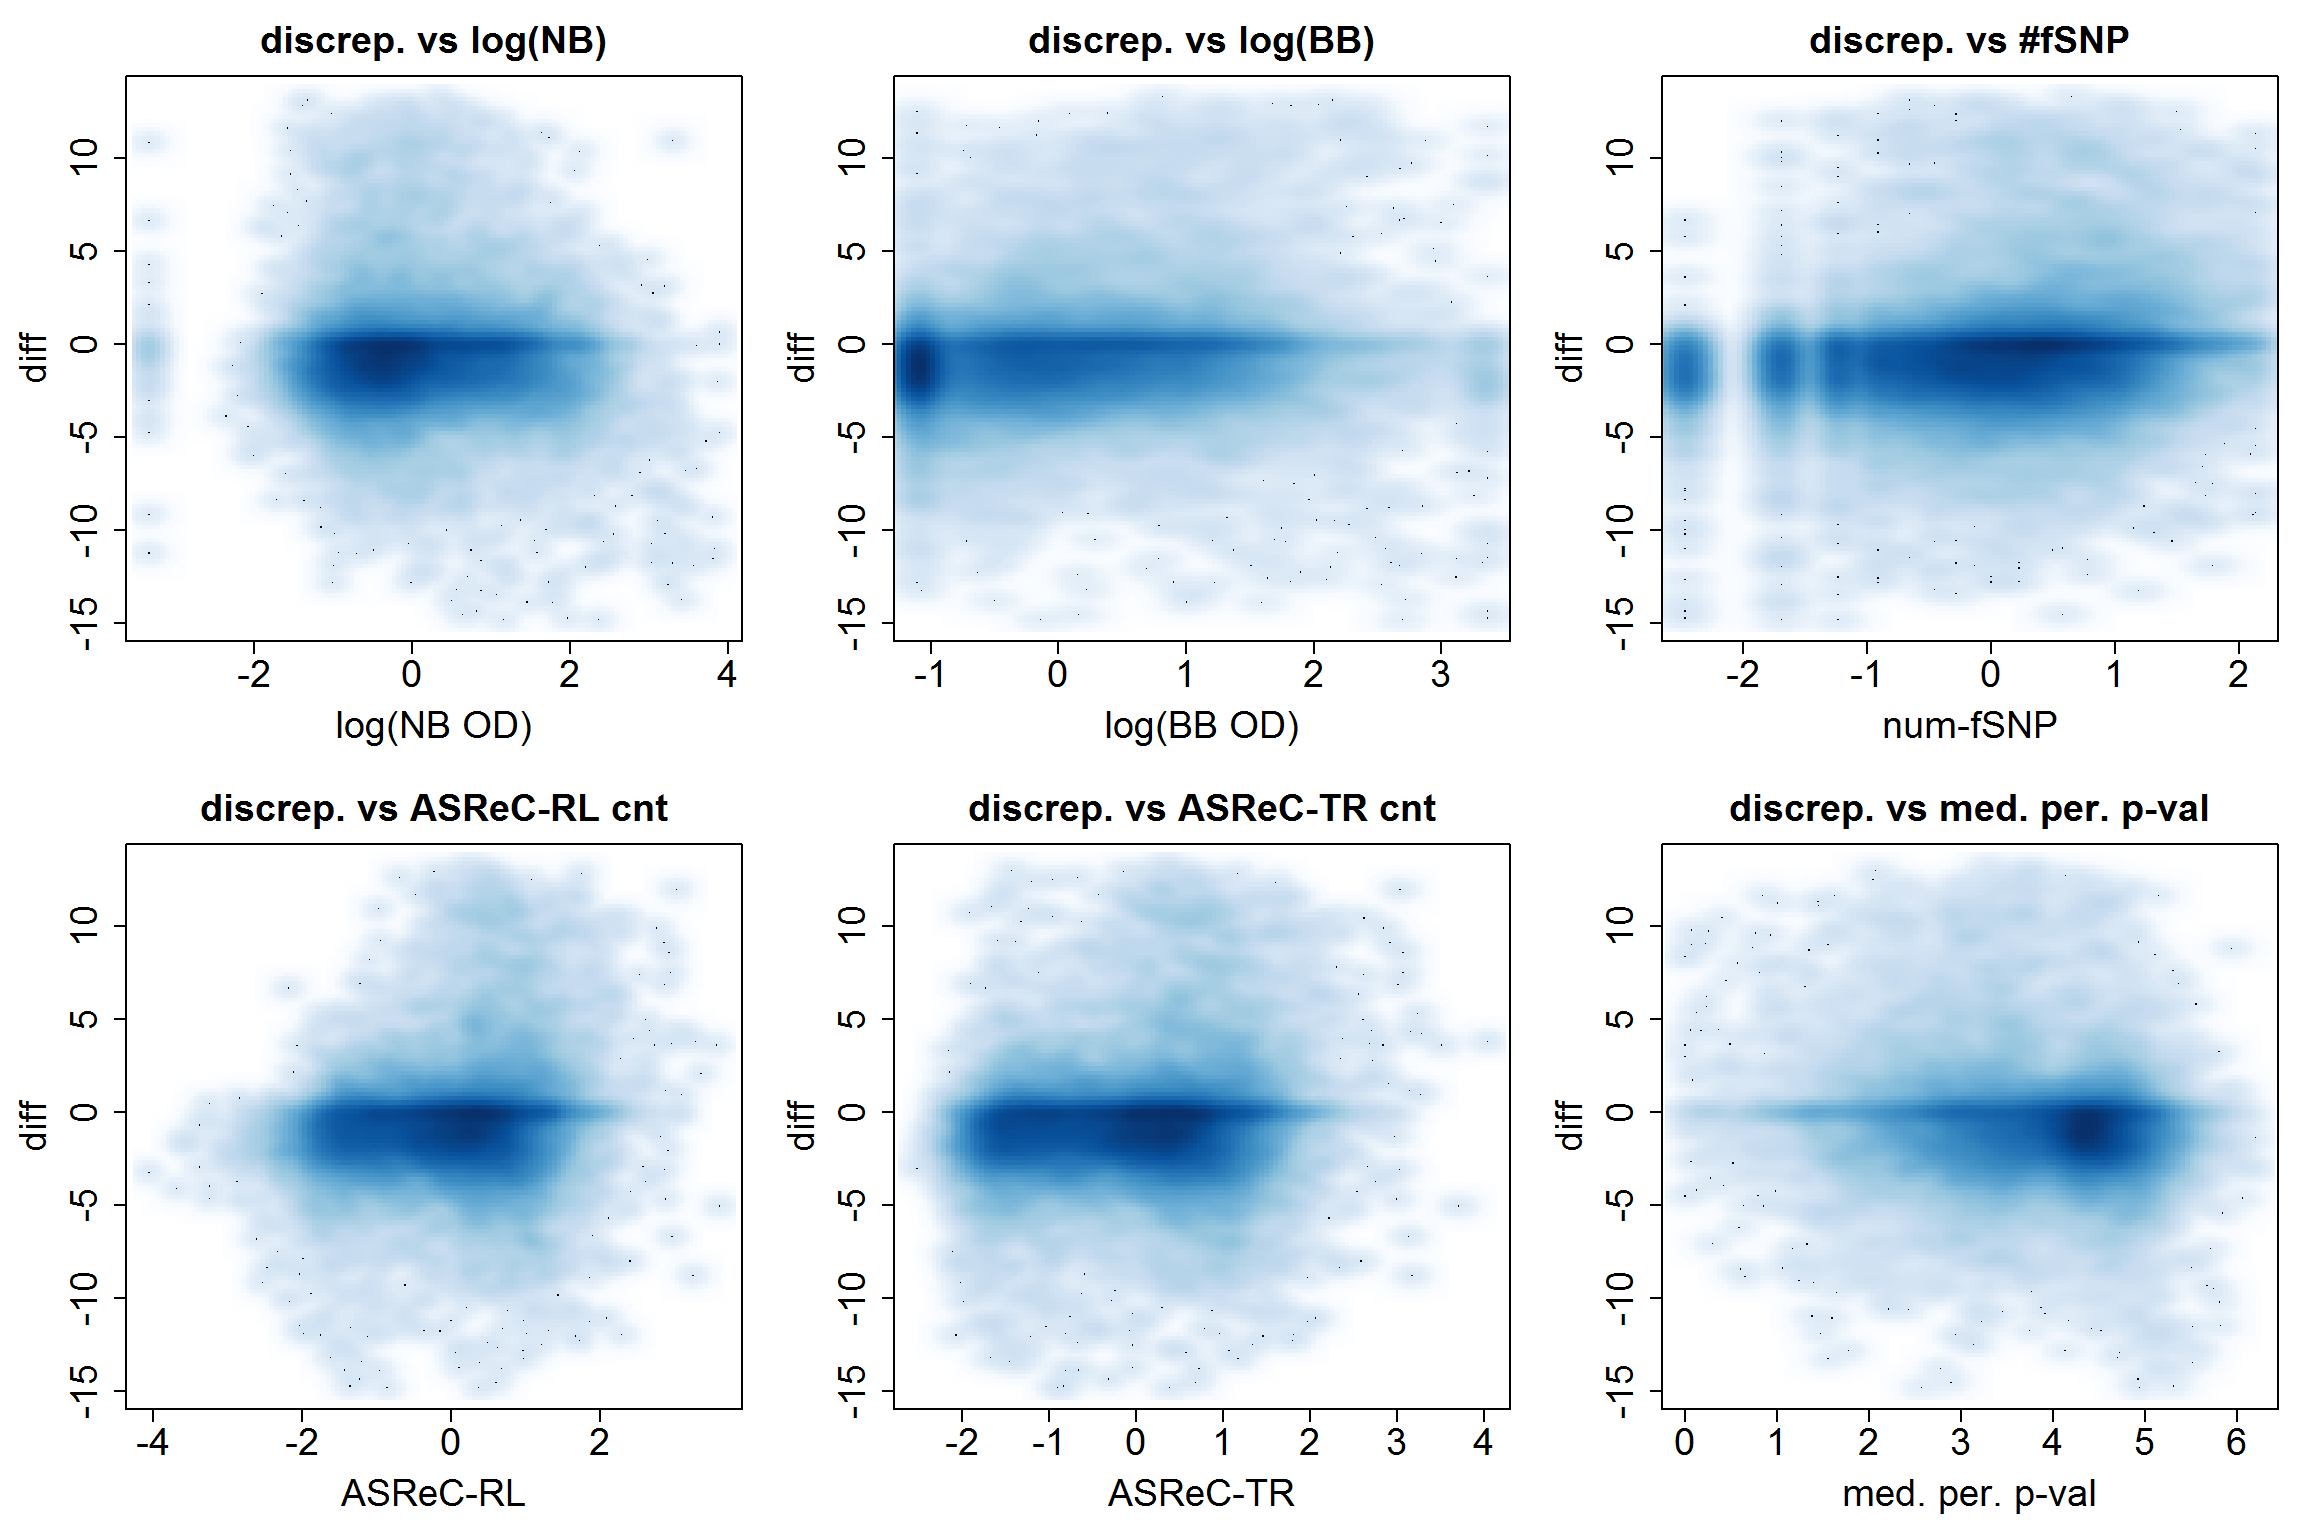
\includegraphics{markdown_files/figure-latex/fig6-1} \end{center}

Adding a wrapper to linear model and anova processing to be run with a
subset of the genes.

Fitting all 13978 genes

\begin{Shaded}
\begin{Highlighting}[]
\CommentTok{#with several cutoffs}
\CommentTok{#kp = abs(y)>=(cutoff-5)}
\NormalTok{cutsub =}\StringTok{ }\DecValTok{0}
\NormalTok{kp =}\StringTok{ }\KeywordTok{abs}\NormalTok{(y)}\OperatorTok{>=}\NormalTok{cutsub}
\KeywordTok{sum}\NormalTok{(kp)}
\end{Highlighting}
\end{Shaded}

\begin{verbatim}
## [1] 13973
\end{verbatim}

\begin{Shaded}
\begin{Highlighting}[]
\NormalTok{resA =}\StringTok{ }\KeywordTok{subset_fit}\NormalTok{(kp, }\DataTypeTok{digits=}\DecValTok{3}\NormalTok{)}
\end{Highlighting}
\end{Shaded}

\begin{verbatim}
## Loading required package: carData
\end{verbatim}

\begin{Shaded}
\begin{Highlighting}[]
\NormalTok{resA}\OperatorTok{$}\NormalTok{tab}
\end{Highlighting}
\end{Shaded}

\begin{verbatim}
##                           Est      SE      P-val      Marg.Est Marg.P    
## (Intercept)               "0.078"  "0.141" " 5.8e-01" "0.308"  " 1.6e-43"
## log(OD_BB)                "0.92"   "0.028" "3.0e-224" "0.606"  "1.5e-168"
## ASReC_R                   "0.806"  "0.062" " 3.0e-38" "0.198"  " 3.8e-19"
## n-fSNP                    "0.439"  "0.027" " 1.6e-60" "0.429"  " 3.6e-84"
## ASReC_R:n-fSNP            "0.239"  "0.024" " 1.1e-23" "0.013"  " 5.1e-01"
## ASReC_R:log(OD_BB)        "0.494"  "0.023" " 1.4e-98" "0.249"  " 1.9e-39"
## n-fSNP:log(OD_BB)         "0.292"  "0.023" " 1.7e-37" "0.133"  " 1.7e-12"
## ASReC_R:n-fSNP:log(OD_BB) "0.111"  "0.017" " 6.9e-11" "-0.046" " 3.9e-04"
## n-rSNP                    "-0.008" "0.022" " 7.1e-01" "0.262"  " 6.2e-32"
## log(OD_NB)                "-0.041" "0.027" " 1.4e-01" "0.262"  " 2.8e-32"
## ASReC_T                   "-0.446" "0.057" " 8.7e-15" "0.084"  " 1.5e-04"
## ASReC_T:ASReC_R           "0.126"  "0.02"  " 1.7e-10" "0.037"  " 4.8e-02"
## AF                        "-0.067" "0.02"  " 9.4e-04" "-0.044" " 4.6e-02"
## Chi2-HWEC                 "-0.115" "0.02"  " 1.8e-08" "-0.155" " 3.0e-12"
## Map.Err                   "-0.016" "0.024" " 5.1e-01" "0.279"  " 2.0e-36"
## Ref.Bias                  "0.247"  "0.026" " 5.6e-22" "0.376"  " 5.5e-65"
## Med(perm-p)               "0.01"   "0.034" " 7.7e-01" "-0.161" " 4.6e-13"
\end{verbatim}

\begin{Shaded}
\begin{Highlighting}[]
\NormalTok{resA}\OperatorTok{$}\NormalTok{ano}
\end{Highlighting}
\end{Shaded}

\begin{verbatim}
##                           SumSq Typ1per  T1P-val Typ3per  T3P-val Marg.R
## log(OD_BB)                 5138     5.3 2.5e-191     6.3 3.0e-224    5.3
## ASReC_R                    2638     2.7 1.1e-100       1  3.0e-38    0.6
## n-fSNP                     1799     1.9  1.3e-69     1.6  1.6e-60    2.7
## ASReC_R:n-fSNP              405     0.4  4.4e-17     0.6  1.1e-23    0.0
## ASReC_R:log(OD_BB)         4109     4.3 2.5e-154     2.7  1.4e-98    1.2
## n-fSNP:log(OD_BB)           755     0.8  2.0e-30       1  1.7e-37    0.4
## ASReC_R:n-fSNP:log(OD_BB)   183     0.2  1.5e-08     0.3  6.9e-11    0.1
## n-rSNP                        0     0.0  9.9e-01       0  7.1e-01    1.0
## log(OD_NB)                    5     0.0  3.3e-01       0  1.4e-01    1.0
## ASReC_T                     322     0.3  6.9e-14     0.4  8.7e-15    0.1
## ASReC_T:ASReC_R             308     0.3  2.2e-13     0.2  1.7e-10    0.0
## AF                           54     0.1  2.2e-03     0.1  9.4e-04    0.0
## Chi2-HWEC                   192     0.2  6.8e-09     0.2  1.8e-08    0.3
## Map.Err                      58     0.1  1.4e-03       0  5.1e-01    1.1
## Ref.Bias                    533     0.6  5.6e-22     0.6  5.6e-22    2.1
## Med(perm-p)                   0     0.0  7.7e-01       0  7.7e-01    0.4
\end{verbatim}

\begin{Shaded}
\begin{Highlighting}[]
\NormalTok{resA}\OperatorTok{$}\NormalTok{r2}
\end{Highlighting}
\end{Shaded}

\begin{verbatim}
## [1] 0.1712933
\end{verbatim}

\begin{Shaded}
\begin{Highlighting}[]
\KeywordTok{write.csv}\NormalTok{(resA}\OperatorTok{$}\NormalTok{ano, }\KeywordTok{sprintf}\NormalTok{(}\StringTok{"anova_cut%s.csv"}\NormalTok{, cutsub), }\DataTypeTok{quote=}\NormalTok{F)}
\KeywordTok{write.csv}\NormalTok{(resA}\OperatorTok{$}\NormalTok{tab, }\KeywordTok{sprintf}\NormalTok{(}\StringTok{"model_cut%s.csv"}\NormalTok{, cutsub), }\DataTypeTok{quote=}\NormalTok{F)}
\end{Highlighting}
\end{Shaded}

Less stringent cutoff (1202 genes)

\begin{Shaded}
\begin{Highlighting}[]
\NormalTok{cutsub =}\StringTok{ }\DecValTok{5}
\NormalTok{kp =}\StringTok{ }\KeywordTok{abs}\NormalTok{(y)}\OperatorTok{>=}\NormalTok{cutsub}
\KeywordTok{sum}\NormalTok{(kp)}
\end{Highlighting}
\end{Shaded}

\begin{verbatim}
## [1] 1019
\end{verbatim}

\begin{Shaded}
\begin{Highlighting}[]
\NormalTok{resA =}\StringTok{ }\KeywordTok{subset_fit}\NormalTok{(kp)}

\NormalTok{resA}\OperatorTok{$}\NormalTok{tab}
\end{Highlighting}
\end{Shaded}

\begin{verbatim}
##                           Est      SE      P-val     Marg.Est Marg.P   
## (Intercept)               "1.037"  "1.054" "3.3e-01" "4.572"  "1.8e-82"
## log(OD_BB)                "3.036"  "0.243" "1.9e-33" "3.244"  "2.7e-64"
## ASReC_R                   "2.445"  "0.503" "1.4e-06" "-0.408" "1.0e-01"
## n-fSNP                    "2.071"  "0.318" "1.2e-10" "1.755"  "8.3e-14"
## ASReC_R:n-fSNP            "0.248"  "0.265" "3.5e-01" "0.745"  "2.2e-04"
## ASReC_R:log(OD_BB)        "1"      "0.205" "1.3e-06" "2.136"  "1.9e-32"
## n-fSNP:log(OD_BB)         "-0.486" "0.2"   "1.5e-02" "0.28"   "1.6e-01"
## ASReC_R:n-fSNP:log(OD_BB) "-0.147" "0.167" "3.8e-01" "-0.16"  "3.4e-01"
## n-rSNP                    "-0.219" "0.209" "3.0e-01" "0.781"  "9.3e-04"
## log(OD_NB)                "-0.98"  "0.229" "2.0e-05" "0.706"  "1.5e-03"
## ASReC_T                   "-2.408" "0.424" "1.8e-08" "-0.852" "1.3e-04"
## ASReC_T:ASReC_R           "0.184"  "0.163" "2.6e-01" "-0.29"  "3.5e-02"
## AF                        "-0.562" "0.18"  "1.8e-03" "-0.839" "1.6e-04"
## Chi2-HWEC                 "-0.22"  "0.185" "2.3e-01" "-0.148" "5.2e-01"
## Map.Err                   "-0.224" "0.163" "1.7e-01" "0.622"  "1.3e-04"
## Ref.Bias                  "0.201"  "0.183" "2.7e-01" "1.194"  "6.3e-12"
## Med(perm-p)               "0.632"  "0.257" "1.4e-02" "0.458"  "1.6e-02"
\end{verbatim}

\begin{Shaded}
\begin{Highlighting}[]
\NormalTok{resA}\OperatorTok{$}\NormalTok{ano}
\end{Highlighting}
\end{Shaded}

\begin{verbatim}
##                           SumSq Typ1per T1P-val Typ3per T3P-val Marg.R
## log(OD_BB)                11936    24.6 9.8e-75     9.7 1.9e-33   24.6
## ASReC_R                     743     1.5 7.7e-07     1.5 1.4e-06    0.3
## n-fSNP                     2166     4.5 7.3e-17     2.6 1.2e-10    5.3
## ASReC_R:n-fSNP               29     0.1 3.3e-01     0.1 3.5e-01    1.3
## ASReC_R:log(OD_BB)          989     2.0 1.3e-08     1.5 1.3e-06   12.9
## n-fSNP:log(OD_BB)           310     0.6 1.4e-03     0.4 1.5e-02    0.2
## ASReC_R:n-fSNP:log(OD_BB)     8     0.0 6.1e-01       0 3.8e-01    0.1
## n-rSNP                      108     0.2 5.9e-02     0.1 3.0e-01    1.1
## log(OD_NB)                  436     0.9 1.5e-04     1.1 2.0e-05    1.0
## ASReC_T                    1043     2.1 5.2e-09       2 1.8e-08    1.4
## ASReC_T:ASReC_R              88     0.2 8.7e-02     0.1 2.6e-01    0.4
## AF                          322     0.7 1.1e-03     0.6 1.8e-03    1.4
## Chi2-HWEC                    57     0.1 1.7e-01     0.1 2.3e-01    0.0
## Map.Err                      21     0.0 4.0e-01     0.1 1.7e-01    1.4
## Ref.Bias                     45     0.1 2.2e-01     0.1 2.7e-01    4.5
## Med(perm-p)                 182     0.4 1.4e-02     0.4 1.4e-02    0.6
\end{verbatim}

\begin{Shaded}
\begin{Highlighting}[]
\NormalTok{resA}\OperatorTok{$}\NormalTok{r2}
\end{Highlighting}
\end{Shaded}

\begin{verbatim}
## [1] 0.3804706
\end{verbatim}

\begin{Shaded}
\begin{Highlighting}[]
\KeywordTok{write.csv}\NormalTok{(resA}\OperatorTok{$}\NormalTok{ano, }\KeywordTok{sprintf}\NormalTok{(}\StringTok{"anova_cut%s.csv"}\NormalTok{, cutsub), }\DataTypeTok{quote=}\NormalTok{F)}
\KeywordTok{write.csv}\NormalTok{(resA}\OperatorTok{$}\NormalTok{tab, }\KeywordTok{sprintf}\NormalTok{(}\StringTok{"model_cut%s.csv"}\NormalTok{, cutsub), }\DataTypeTok{quote=}\NormalTok{F)}
\end{Highlighting}
\end{Shaded}

The most discrepant 221 genes

\begin{Shaded}
\begin{Highlighting}[]
\NormalTok{cutsub =}\StringTok{ }\NormalTok{cutoff}\OperatorTok{-}\DecValTok{5}
\NormalTok{kp =}\StringTok{ }\KeywordTok{abs}\NormalTok{(y)}\OperatorTok{>=}\NormalTok{cutsub}
\KeywordTok{sum}\NormalTok{(kp)}
\end{Highlighting}
\end{Shaded}

\begin{verbatim}
## [1] 235
\end{verbatim}

\begin{Shaded}
\begin{Highlighting}[]
\NormalTok{resA =}\StringTok{ }\KeywordTok{subset_fit}\NormalTok{(kp)}

\NormalTok{resA}\OperatorTok{$}\NormalTok{tab}
\end{Highlighting}
\end{Shaded}

\begin{verbatim}
##                           Est      SE      P-val     Marg.Est Marg.P   
## (Intercept)               "6.408"  "1.97"  "1.3e-03" "9.717"  "1.3e-68"
## log(OD_BB)                "1.502"  "0.461" "1.3e-03" "1.995"  "1.4e-08"
## ASReC_R                   "-0.811" "0.973" "4.1e-01" "-1.038" "4.4e-02"
## n-fSNP                    "1.629"  "0.803" "4.4e-02" "1.106"  "1.3e-02"
## ASReC_R:n-fSNP            "1.186"  "0.747" "1.1e-01" "0.67"   "9.4e-02"
## ASReC_R:log(OD_BB)        "1.504"  "0.442" "7.9e-04" "1.521"  "4.5e-06"
## n-fSNP:log(OD_BB)         "-0.413" "0.466" "3.8e-01" "-0.084" "8.0e-01"
## ASReC_R:n-fSNP:log(OD_BB) "-0.385" "0.499" "4.4e-01" "-0.151" "6.6e-01"
## n-rSNP                    "-0.807" "0.372" "3.1e-02" "-0.162" "6.9e-01"
## log(OD_NB)                "-0.735" "0.419" "8.1e-02" "-0.183" "6.6e-01"
## ASReC_T                   "-1.998" "0.718" "5.9e-03" "-1.019" "1.5e-02"
## ASReC_T:ASReC_R           "0.68"   "0.379" "7.4e-02" "-0.324" "1.9e-01"
## AF                        "-0.399" "0.352" "2.6e-01" "-0.756" "4.9e-02"
## Chi2-HWEC                 "-0.149" "0.388" "7.0e-01" "0.202"  "6.3e-01"
## Map.Err                   "-0.241" "0.27"  "3.7e-01" "-0.102" "6.9e-01"
## Ref.Bias                  "-0.283" "0.315" "3.7e-01" "0.283"  "3.3e-01"
## Med(perm-p)               "0.95"   "0.479" "4.9e-02" "0.871"  "1.9e-02"
\end{verbatim}

\begin{Shaded}
\begin{Highlighting}[]
\NormalTok{resA}\OperatorTok{$}\NormalTok{ano}
\end{Highlighting}
\end{Shaded}

\begin{verbatim}
##                           SumSq Typ1per T1P-val Typ3per T3P-val Marg.R
## log(OD_BB)                 1058    12.9 5.5e-10     3.3 1.3e-03   12.9
## ASReC_R                      14     0.2 4.5e-01     0.2 4.1e-01    1.7
## n-fSNP                      472     5.8 2.2e-05     1.3 4.4e-02    2.6
## ASReC_R:n-fSNP                0     0.0 8.9e-01     0.8 1.1e-01    1.2
## ASReC_R:log(OD_BB)          336     4.1 3.2e-04     3.6 7.9e-04    8.7
## n-fSNP:log(OD_BB)           124     1.5 2.7e-02     0.2 3.8e-01    0.0
## ASReC_R:n-fSNP:log(OD_BB)    31     0.4 2.7e-01     0.2 4.4e-01    0.1
## n-rSNP                      123     1.5 2.8e-02     1.4 3.1e-02    0.1
## log(OD_NB)                   69     0.8 9.9e-02     0.9 8.1e-02    0.1
## ASReC_T                     164     2.0 1.1e-02     2.4 5.9e-03    2.5
## ASReC_T:ASReC_R             106     1.3 4.1e-02       1 7.4e-02    0.7
## AF                           67     0.8 1.0e-01     0.4 2.6e-01    1.7
## Chi2-HWEC                     2     0.0 8.0e-01       0 7.0e-01    0.1
## Map.Err                      34     0.4 2.4e-01     0.2 3.7e-01    0.1
## Ref.Bias                     11     0.1 5.1e-01     0.2 3.7e-01    0.4
## Med(perm-p)                  99     1.2 4.9e-02     1.2 4.9e-02    2.4
\end{verbatim}

\begin{Shaded}
\begin{Highlighting}[]
\NormalTok{resA}\OperatorTok{$}\NormalTok{r2}
\end{Highlighting}
\end{Shaded}

\begin{verbatim}
## [1] 0.3313608
\end{verbatim}

\begin{Shaded}
\begin{Highlighting}[]
\KeywordTok{write.csv}\NormalTok{(resA}\OperatorTok{$}\NormalTok{ano, }\KeywordTok{sprintf}\NormalTok{(}\StringTok{"anova_cut%s.csv"}\NormalTok{, cutsub), }\DataTypeTok{quote=}\NormalTok{F)}
\KeywordTok{write.csv}\NormalTok{(resA}\OperatorTok{$}\NormalTok{tab, }\KeywordTok{sprintf}\NormalTok{(}\StringTok{"model_cut%s.csv"}\NormalTok{, cutsub), }\DataTypeTok{quote=}\NormalTok{F)}
\end{Highlighting}
\end{Shaded}

plot(lodNB{[}kp{]}, y{[}kp{]}, main=``discrep. vs log(NB)'',
ylab=``diff'', cex=0.5, col=rgb(0.8,0.1,0.1,0.5), xlab=``log(NB OD)'',
cex.main=cexes, cex.lab=cexes, cex.axis=cexes, pch=20)

Keeping only genes with difference \textless{}10

\begin{Shaded}
\begin{Highlighting}[]
\NormalTok{cutsub =}\StringTok{ }\DecValTok{10}
\NormalTok{kp =}\StringTok{ }\KeywordTok{abs}\NormalTok{(y)}\OperatorTok{<}\NormalTok{cutsub}
\KeywordTok{sum}\NormalTok{(kp)}
\end{Highlighting}
\end{Shaded}

\begin{verbatim}
## [1] 13738
\end{verbatim}

\begin{Shaded}
\begin{Highlighting}[]
\NormalTok{resA =}\StringTok{ }\KeywordTok{subset_fit}\NormalTok{(kp)}

\NormalTok{resA}\OperatorTok{$}\NormalTok{tab}
\end{Highlighting}
\end{Shaded}

\begin{verbatim}
##                           Est      SE      P-val      Marg.Est Marg.P    
## (Intercept)               "-0.024" "0.122" " 8.4e-01" "0.147"  " 5.6e-15"
## log(OD_BB)                "0.689"  "0.025" "3.0e-164" "0.465"  "9.3e-136"
## ASReC_R                   "0.567"  "0.054" " 2.4e-25" "0.082"  " 1.4e-05"
## n-fSNP                    "0.379"  "0.023" " 5.7e-60" "0.372"  " 1.9e-88"
## ASReC_R:n-fSNP            "0.199"  "0.021" " 4.6e-22" "0.012"  " 4.5e-01"
## ASReC_R:log(OD_BB)        "0.347"  "0.02"  " 3.8e-64" "0.139"  " 7.0e-18"
## n-fSNP:log(OD_BB)         "0.241"  "0.02"  " 1.9e-33" "0.12"   " 5.3e-14"
## ASReC_R:n-fSNP:log(OD_BB) "0.074"  "0.015" " 5.1e-07" "-0.047" " 1.7e-05"
## n-rSNP                    "0.038"  "0.019" " 4.6e-02" "0.268"  " 1.3e-45"
## log(OD_NB)                "0.029"  "0.024" " 2.3e-01" "0.288"  " 2.1e-53"
## ASReC_T                   "-0.337" "0.05"  " 2.4e-11" "-0.004" " 8.5e-01"
## ASReC_T:ASReC_R           "0.106"  "0.017" " 6.5e-10" "0.052"  " 1.4e-03"
## AF                        "-0.038" "0.018" " 2.8e-02" "-0.014" " 4.7e-01"
## Chi2-HWEC                 "-0.124" "0.018" " 1.7e-12" "-0.167" " 7.6e-19"
## Map.Err                   "-0.021" "0.021" " 3.2e-01" "0.172"  " 2.5e-19"
## Ref.Bias                  "0.149"  "0.022" " 2.9e-11" "0.246"  " 2.4e-38"
## Med(perm-p)               "0.012"  "0.03"  " 6.8e-01" "-0.094" " 6.0e-07"
\end{verbatim}

\begin{Shaded}
\begin{Highlighting}[]
\NormalTok{resA}\OperatorTok{$}\NormalTok{ano}
\end{Highlighting}
\end{Shaded}

\begin{verbatim}
##                           SumSq Typ1per  T1P-val Typ3per  T3P-val Marg.R
## log(OD_BB)                 2933     4.4 3.6e-150     4.8 3.0e-164    4.4
## ASReC_R                     975     1.5  5.5e-52     0.7  2.4e-25    0.1
## n-fSNP                     1667     2.5  4.3e-87     1.7  5.7e-60    2.9
## ASReC_R:n-fSNP              240     0.4  4.1e-14     0.6  4.6e-22    0.0
## ASReC_R:log(OD_BB)         1997     3.0 1.2e-103     1.8  3.8e-64    0.5
## n-fSNP:log(OD_BB)           599     0.9  9.7e-33     0.9  1.9e-33    0.4
## ASReC_R:n-fSNP:log(OD_BB)    68     0.1  5.9e-05     0.2  5.1e-07    0.1
## n-rSNP                       39     0.1  2.4e-03       0  4.6e-02    1.5
## log(OD_NB)                   53     0.1  4.1e-04       0  2.3e-01    1.7
## ASReC_T                     170     0.3  2.1e-10     0.3  2.4e-11    0.0
## ASReC_T:ASReC_R             198     0.3  6.5e-12     0.2  6.5e-10    0.1
## AF                           18     0.0  4.0e-02       0  2.8e-02    0.0
## Chi2-HWEC                   216     0.3  7.6e-13     0.3  1.7e-12    0.6
## Map.Err                      10     0.0  1.2e-01       0  3.2e-01    0.6
## Ref.Bias                    186     0.3  3.0e-11     0.3  2.9e-11    1.2
## Med(perm-p)                   1     0.0  6.8e-01       0  6.8e-01    0.2
\end{verbatim}

\begin{Shaded}
\begin{Highlighting}[]
\NormalTok{resA}\OperatorTok{$}\NormalTok{r2}
\end{Highlighting}
\end{Shaded}

\begin{verbatim}
## [1] 0.139862
\end{verbatim}

\begin{Shaded}
\begin{Highlighting}[]
\KeywordTok{write.csv}\NormalTok{(resA}\OperatorTok{$}\NormalTok{ano, }\KeywordTok{sprintf}\NormalTok{(}\StringTok{"anova_less%s.csv"}\NormalTok{, cutsub), }\DataTypeTok{quote=}\NormalTok{F)}
\KeywordTok{write.csv}\NormalTok{(resA}\OperatorTok{$}\NormalTok{tab, }\KeywordTok{sprintf}\NormalTok{(}\StringTok{"model_less%s.csv"}\NormalTok{, cutsub), }\DataTypeTok{quote=}\NormalTok{F)}
\end{Highlighting}
\end{Shaded}

Keeping only genes with difference \textless{}5

\begin{Shaded}
\begin{Highlighting}[]
\NormalTok{cutsub =}\StringTok{ }\DecValTok{5}
\NormalTok{kp =}\StringTok{ }\KeywordTok{abs}\NormalTok{(y)}\OperatorTok{<}\NormalTok{cutsub}
\KeywordTok{sum}\NormalTok{(kp)}
\end{Highlighting}
\end{Shaded}

\begin{verbatim}
## [1] 12954
\end{verbatim}

\begin{Shaded}
\begin{Highlighting}[]
\NormalTok{resA =}\StringTok{ }\KeywordTok{subset_fit}\NormalTok{(kp)}

\NormalTok{resA}\OperatorTok{$}\NormalTok{tab}
\end{Highlighting}
\end{Shaded}

\begin{verbatim}
##                           Est      SE      P-val     Marg.Est Marg.P   
## (Intercept)               "-0.032" "0.087" "7.1e-01" "-0.027" "3.5e-02"
## log(OD_BB)                "0.363"  "0.018" "2.8e-90" "0.264"  "1.9e-93"
## ASReC_R                   "0.273"  "0.038" "1.4e-12" "-0.022" "9.3e-02"
## n-fSNP                    "0.21"   "0.016" "4.8e-38" "0.207"  "1.4e-58"
## ASReC_R:n-fSNP            "0.082"  "0.015" "2.3e-08" "-0.014" "2.0e-01"
## ASReC_R:log(OD_BB)        "0.152"  "0.015" "2.1e-24" "0.019"  "8.1e-02"
## n-fSNP:log(OD_BB)         "0.115"  "0.014" "1.8e-15" "0.056"  "2.5e-07"
## ASReC_R:n-fSNP:log(OD_BB) "0.023"  "0.011" "3.0e-02" "-0.031" "2.2e-05"
## n-rSNP                    "0.028"  "0.013" "3.3e-02" "0.156"  "4.8e-34"
## log(OD_NB)                "0.072"  "0.017" "1.6e-05" "0.223"  "1.6e-68"
## ASReC_T                   "-0.199" "0.036" "2.4e-08" "-0.071" "6.4e-08"
## ASReC_T:ASReC_R           "0.066"  "0.013" "2.0e-07" "0.047"  "4.1e-05"
## AF                        "-0.005" "0.012" "7.0e-01" "0.014"  "2.8e-01"
## Chi2-HWEC                 "-0.094" "0.012" "1.7e-14" "-0.12"  "8.7e-21"
## Map.Err                   "-0.044" "0.015" "3.9e-03" "0.05"   "1.9e-04"
## Ref.Bias                  "0.065"  "0.016" "4.4e-05" "0.118"  "4.6e-19"
## Med(perm-p)               "-0.012" "0.021" "5.6e-01" "-0.011" "3.9e-01"
\end{verbatim}

\begin{Shaded}
\begin{Highlighting}[]
\NormalTok{resA}\OperatorTok{$}\NormalTok{ano}
\end{Highlighting}
\end{Shaded}

\begin{verbatim}
##                           SumSq Typ1per T1P-val Typ3per T3P-val Marg.R
## log(OD_BB)                  887     3.2 3.2e-99     2.9 2.8e-90    3.2
## ASReC_R                      88     0.3 2.0e-11     0.4 1.4e-12    0.0
## n-fSNP                      642     2.3 1.1e-72     1.2 4.8e-38    2.0
## ASReC_R:n-fSNP               22     0.1 7.7e-04     0.2 2.3e-08    0.0
## ASReC_R:log(OD_BB)          350     1.3 1.1e-40     0.7 2.1e-24    0.0
## n-fSNP:log(OD_BB)           176     0.6 2.8e-21     0.4 1.8e-15    0.2
## ASReC_R:n-fSNP:log(OD_BB)     2     0.0 3.2e-01       0 3.0e-02    0.1
## n-rSNP                       25     0.1 3.1e-04       0 3.3e-02    1.1
## log(OD_NB)                   74     0.3 7.8e-10     0.1 1.6e-05    2.3
## ASReC_T                      54     0.2 1.6e-07     0.2 2.4e-08    0.2
## ASReC_T:ASReC_R              62     0.2 1.6e-08     0.2 2.0e-07    0.1
## AF                            0     0.0 7.8e-01       0 7.0e-01    0.0
## Chi2-HWEC                   117     0.4 1.0e-14     0.4 1.7e-14    0.7
## Map.Err                       5     0.0 1.2e-01     0.1 3.9e-03    0.1
## Ref.Bias                     33     0.1 4.3e-05     0.1 4.4e-05    0.6
## Med(perm-p)                   1     0.0 5.6e-01       0 5.6e-01    0.0
\end{verbatim}

\begin{Shaded}
\begin{Highlighting}[]
\NormalTok{resA}\OperatorTok{$}\NormalTok{r2}
\end{Highlighting}
\end{Shaded}

\begin{verbatim}
## [1] 0.09138135
\end{verbatim}

\begin{Shaded}
\begin{Highlighting}[]
\KeywordTok{write.csv}\NormalTok{(resA}\OperatorTok{$}\NormalTok{ano, }\KeywordTok{sprintf}\NormalTok{(}\StringTok{"anova_less%s.csv"}\NormalTok{, cutsub), }\DataTypeTok{quote=}\NormalTok{F)}
\KeywordTok{write.csv}\NormalTok{(resA}\OperatorTok{$}\NormalTok{tab, }\KeywordTok{sprintf}\NormalTok{(}\StringTok{"model_less%s.csv"}\NormalTok{, cutsub), }\DataTypeTok{quote=}\NormalTok{F)}
\end{Highlighting}
\end{Shaded}

\begin{Shaded}
\begin{Highlighting}[]
\NormalTok{kp =}\StringTok{ }\KeywordTok{abs}\NormalTok{(y)}\OperatorTok{>}\DecValTok{5}
\NormalTok{lm.r =}\StringTok{ }\KeywordTok{lm}\NormalTok{(lodR[kp]}\OperatorTok{~}\NormalTok{lodBB[kp]}\OperatorTok{+}\NormalTok{lodNB[kp]}\OperatorTok{+}\NormalTok{lodBB[kp]}\OperatorTok{:}\NormalTok{lodNB[kp])}
\NormalTok{odr =}\StringTok{ }\NormalTok{lm.r}\OperatorTok{$}\NormalTok{residuals}
\NormalTok{lm.}\DecValTok{3}\NormalTok{ =}\StringTok{ }\KeywordTok{lm}\NormalTok{(y[kp]}\OperatorTok{~}\NormalTok{lodBB[kp]}\OperatorTok{+}\NormalTok{asR[kp]}\OperatorTok{+}\NormalTok{NfSNP[kp]}
             \OperatorTok{+}\NormalTok{i12[kp]}\OperatorTok{+}\NormalTok{i13[kp]}\OperatorTok{+}\NormalTok{i23[kp]}\OperatorTok{+}\NormalTok{i123[kp]}
             \OperatorTok{+}\NormalTok{NrSNP[kp]}\OperatorTok{+}\NormalTok{lodNB[kp]}\OperatorTok{+}\NormalTok{asT[kp]}\OperatorTok{+}\NormalTok{ia14[kp]}\OperatorTok{+}\NormalTok{odr}
             \OperatorTok{+}\NormalTok{af[kp]}\OperatorTok{+}\NormalTok{hwec2[kp]}\OperatorTok{+}\NormalTok{derr[kp]}\OperatorTok{+}\NormalTok{phib[kp]}\OperatorTok{+}\NormalTok{mpp[kp])}
\KeywordTok{summary}\NormalTok{(lm.}\DecValTok{3}\NormalTok{)}
\end{Highlighting}
\end{Shaded}

\begin{verbatim}
## 
## Call:
## lm(formula = y[kp] ~ lodBB[kp] + asR[kp] + NfSNP[kp] + i12[kp] + 
##     i13[kp] + i23[kp] + i123[kp] + NrSNP[kp] + lodNB[kp] + asT[kp] + 
##     ia14[kp] + odr + af[kp] + hwec2[kp] + derr[kp] + phib[kp] + 
##     mpp[kp])
## 
## Residuals:
##      Min       1Q   Median       3Q      Max 
## -21.1025  -3.4561   0.9201   3.6510  12.3166 
## 
## Coefficients:
##             Estimate Std. Error t value Pr(>|t|)    
## (Intercept)  1.25809    1.05231   1.196  0.23216    
## lodBB[kp]    3.26973    0.25289  12.929  < 2e-16 ***
## asR[kp]      2.72741    0.50891   5.359 1.04e-07 ***
## NfSNP[kp]    1.93531    0.31993   6.049 2.05e-09 ***
## i12[kp]      0.26262    0.26419   0.994  0.32044    
## i13[kp]      0.92699    0.20568   4.507 7.35e-06 ***
## i23[kp]     -0.52715    0.19919  -2.646  0.00826 ** 
## i123[kp]    -0.15993    0.16641  -0.961  0.33677    
## NrSNP[kp]   -0.19214    0.20850  -0.922  0.35699    
## lodNB[kp]   -0.93538    0.22831  -4.097 4.53e-05 ***
## asT[kp]     -2.54535    0.42449  -5.996 2.82e-09 ***
## ia14[kp]     0.26871    0.16477   1.631  0.10324    
## odr          1.17698    0.37324   3.153  0.00166 ** 
## af[kp]      -0.52496    0.17938  -2.927  0.00351 ** 
## hwec2[kp]   -0.24650    0.18468  -1.335  0.18227    
## derr[kp]    -0.44491    0.17716  -2.511  0.01219 *  
## phib[kp]     0.08762    0.18562   0.472  0.63699    
## mpp[kp]      0.59753    0.25630   2.331  0.01993 *  
## ---
## Signif. codes:  0 '***' 0.001 '**' 0.01 '*' 0.05 '.' 0.1 ' ' 1
## 
## Residual standard error: 5.458 on 1000 degrees of freedom
## Multiple R-squared:  0.3867, Adjusted R-squared:  0.3763 
## F-statistic: 37.09 on 17 and 1000 DF,  p-value: < 2.2e-16
\end{verbatim}

\begin{Shaded}
\begin{Highlighting}[]
\KeywordTok{anova}\NormalTok{(lm.r)}
\end{Highlighting}
\end{Shaded}

\begin{verbatim}
## Analysis of Variance Table
## 
## Response: lodR[kp]
##                       Df Sum Sq Mean Sq   F value Pr(>F)    
## lodBB[kp]              1 442.25  442.25 1327.6702 <2e-16 ***
## lodNB[kp]              1 363.97  363.97 1092.6780 <2e-16 ***
## lodBB[kp]:lodNB[kp]    1   0.31    0.31    0.9251 0.3364    
## Residuals           1014 337.77    0.33                     
## ---
## Signif. codes:  0 '***' 0.001 '**' 0.01 '*' 0.05 '.' 0.1 ' ' 1
\end{verbatim}

\begin{Shaded}
\begin{Highlighting}[]
\KeywordTok{anova}\NormalTok{(lm.}\DecValTok{3}\NormalTok{)}
\end{Highlighting}
\end{Shaded}

\begin{verbatim}
## Analysis of Variance Table
## 
## Response: y[kp]
##             Df  Sum Sq Mean Sq  F value    Pr(>F)    
## lodBB[kp]    1 11936.7 11936.7 400.6745 < 2.2e-16 ***
## asR[kp]      1   742.4   742.4  24.9194 7.049e-07 ***
## NfSNP[kp]    1  2170.7  2170.7  72.8628 < 2.2e-16 ***
## i12[kp]      1    30.2    30.2   1.0136 0.3142792    
## i13[kp]      1   988.4   988.4  33.1769 1.119e-08 ***
## i23[kp]      1   309.5   309.5  10.3879 0.0013095 ** 
## i123[kp]     1     7.8     7.8   0.2604 0.6099271    
## NrSNP[kp]    1   107.0   107.0   3.5932 0.0583059 .  
## lodNB[kp]    1   432.6   432.6  14.5208 0.0001471 ***
## asT[kp]      1  1047.4  1047.4  35.1578 4.183e-09 ***
## ia14[kp]     1    87.3    87.3   2.9316 0.0871721 .  
## odr          1   178.0   178.0   5.9735 0.0146941 *  
## af[kp]       1   322.8   322.8  10.8347 0.0010310 ** 
## hwec2[kp]    1    71.6    71.6   2.4023 0.1214716    
## derr[kp]     1   181.1   181.1   6.0782 0.0138533 *  
## phib[kp]     1     9.6     9.6   0.3236 0.5696024    
## mpp[kp]      1   161.9   161.9   5.4353 0.0199311 *  
## Residuals 1000 29791.4    29.8                       
## ---
## Signif. codes:  0 '***' 0.001 '**' 0.01 '*' 0.05 '.' 0.1 ' ' 1
\end{verbatim}

\begin{Shaded}
\begin{Highlighting}[]
\NormalTok{cexes =}\StringTok{ }\FloatTok{1.2}
\KeywordTok{png}\NormalTok{(}\StringTok{"new_od_plot.png"}\NormalTok{, }\DataTypeTok{height=}\DecValTok{4}\NormalTok{, }\DataTypeTok{width=}\DecValTok{4}\NormalTok{, }\DataTypeTok{res=}\DecValTok{300}\NormalTok{, }\DataTypeTok{units=}\StringTok{"in"}\NormalTok{)}
\KeywordTok{par}\NormalTok{(}\DataTypeTok{mar=}\KeywordTok{c}\NormalTok{(}\DecValTok{5}\NormalTok{,}\DecValTok{5}\NormalTok{,}\DecValTok{3}\NormalTok{,}\DecValTok{1}\NormalTok{))}
\KeywordTok{plot}\NormalTok{(lodNBp, lodBBp, }\DataTypeTok{main=}\StringTok{"NB vs BB over-disp"}\NormalTok{, }\DataTypeTok{pch=}\DecValTok{20}\NormalTok{, }\DataTypeTok{cex=}\NormalTok{.}\DecValTok{5}\NormalTok{, }\DataTypeTok{col=}\KeywordTok{rgb}\NormalTok{(}\FloatTok{0.4}\NormalTok{,}\FloatTok{0.4}\NormalTok{,}\FloatTok{0.4}\NormalTok{,}\FloatTok{0.5}\NormalTok{), }\DataTypeTok{bty=}\StringTok{"n"}\NormalTok{,}
     \DataTypeTok{xlab=}\StringTok{"log10(NB overdispersion)"}\NormalTok{, }\DataTypeTok{ylab=}\StringTok{"log(BB overdispersion)"}\NormalTok{, }\DataTypeTok{cex.main=}\NormalTok{cexes, }\DataTypeTok{cex.lab=}\NormalTok{cexes, }\DataTypeTok{cex.axis=}\NormalTok{cexes)}
\KeywordTok{abline}\NormalTok{(}\DataTypeTok{a=}\DecValTok{0}\NormalTok{, }\DataTypeTok{b=}\DecValTok{1}\NormalTok{, }\DataTypeTok{col=}\StringTok{"red"}\NormalTok{, }\DataTypeTok{lwd=}\DecValTok{2}\NormalTok{, }\DataTypeTok{lty=}\DecValTok{3}\NormalTok{)}
\KeywordTok{dev.off}\NormalTok{()}
\end{Highlighting}
\end{Shaded}

\begin{verbatim}
## pdf 
##   2
\end{verbatim}

\begin{Shaded}
\begin{Highlighting}[]
\NormalTok{rasqS =}\StringTok{ }\NormalTok{trecS =}\StringTok{ }\KeywordTok{rep}\NormalTok{(}\DecValTok{0}\NormalTok{, }\KeywordTok{nrow}\NormalTok{(rasq))}
\NormalTok{rasqS[rasq}\OperatorTok{$}\NormalTok{qvalR}\OperatorTok{<}\FloatTok{5e-2}\NormalTok{] =}\StringTok{ }\DecValTok{1}
\NormalTok{rasqS[rasq}\OperatorTok{$}\NormalTok{qvalR}\OperatorTok{<}\FloatTok{1e-3}\NormalTok{] =}\StringTok{ }\DecValTok{2}
\NormalTok{rasqS[rasq}\OperatorTok{$}\NormalTok{qvalR}\OperatorTok{<}\FloatTok{1e-4}\NormalTok{] =}\StringTok{ }\DecValTok{3}
\NormalTok{rasqS[rasq}\OperatorTok{$}\NormalTok{qvalR}\OperatorTok{<}\FloatTok{1e-5}\NormalTok{] =}\StringTok{ }\DecValTok{4}

\NormalTok{trecS[rasq}\OperatorTok{$}\NormalTok{qvalT}\OperatorTok{<}\FloatTok{5e-2}\NormalTok{] =}\StringTok{ }\DecValTok{1}
\NormalTok{trecS[rasq}\OperatorTok{$}\NormalTok{qvalT}\OperatorTok{<}\FloatTok{1e-3}\NormalTok{] =}\StringTok{ }\DecValTok{2}
\NormalTok{trecS[rasq}\OperatorTok{$}\NormalTok{qvalT}\OperatorTok{<}\FloatTok{1e-4}\NormalTok{] =}\StringTok{ }\DecValTok{3}
\NormalTok{trecS[rasq}\OperatorTok{$}\NormalTok{qvalT}\OperatorTok{<}\FloatTok{1e-5}\NormalTok{] =}\StringTok{ }\DecValTok{4}

\KeywordTok{table}\NormalTok{(rasqS, trecS)}
\end{Highlighting}
\end{Shaded}

\begin{verbatim}
##      trecS
## rasqS    0    1    2    3    4
##     0 3420 1335  210  115  172
##     1  538 1357  484  254  294
##     2   70  279  232  184  292
##     3   38  142  105  124  304
##     4  161  281  190  264 3128
\end{verbatim}

\begin{Shaded}
\begin{Highlighting}[]
\NormalTok{cexes =}\StringTok{ }\FloatTok{1.7}
\KeywordTok{png}\NormalTok{(}\StringTok{"od_vs_rasq_plot.png"}\NormalTok{, }\DataTypeTok{height=}\DecValTok{4}\NormalTok{, }\DataTypeTok{width=}\DecValTok{8}\NormalTok{, }\DataTypeTok{res=}\DecValTok{300}\NormalTok{, }\DataTypeTok{units=}\StringTok{"in"}\NormalTok{)}
\KeywordTok{par}\NormalTok{(}\DataTypeTok{mfrow=}\KeywordTok{c}\NormalTok{(}\DecValTok{1}\NormalTok{,}\DecValTok{2}\NormalTok{))}
\KeywordTok{par}\NormalTok{(}\DataTypeTok{mar=}\KeywordTok{c}\NormalTok{(}\DecValTok{5}\NormalTok{,}\DecValTok{5}\NormalTok{,}\DecValTok{3}\NormalTok{,}\DecValTok{1}\NormalTok{))}
\KeywordTok{plot}\NormalTok{(lodRp, lodNBp, }\DataTypeTok{main=}\StringTok{"(a) RASQUAL vs NB"}\NormalTok{, }\DataTypeTok{pch=}\DecValTok{20}\NormalTok{, }\DataTypeTok{cex=}\NormalTok{.}\DecValTok{5}\NormalTok{, }\DataTypeTok{col=}\KeywordTok{rgb}\NormalTok{(}\FloatTok{0.4}\NormalTok{,}\FloatTok{0.4}\NormalTok{,}\FloatTok{0.4}\NormalTok{,}\FloatTok{0.5}\NormalTok{), }\DataTypeTok{bty=}\StringTok{"n"}\NormalTok{,}
     \DataTypeTok{xlab=}\StringTok{"log10(RASQUAL od)"}\NormalTok{, }\DataTypeTok{ylab=}\StringTok{"log10(TReCASE NB od)"}\NormalTok{, }\DataTypeTok{cex.main=}\NormalTok{cexes, }\DataTypeTok{cex.lab=}\NormalTok{cexes, }\DataTypeTok{cex.axis=}\NormalTok{cexes)}
\KeywordTok{abline}\NormalTok{(}\DataTypeTok{a=}\DecValTok{0}\NormalTok{, }\DataTypeTok{b=}\DecValTok{1}\NormalTok{, }\DataTypeTok{col=}\StringTok{"red"}\NormalTok{, }\DataTypeTok{lwd=}\DecValTok{2}\NormalTok{, }\DataTypeTok{lty=}\DecValTok{3}\NormalTok{)}

\KeywordTok{plot}\NormalTok{(lodRp, lodBBp, }\DataTypeTok{main=}\StringTok{"(b) RASQUAL vs BB"}\NormalTok{, }\DataTypeTok{pch=}\DecValTok{20}\NormalTok{, }\DataTypeTok{cex=}\NormalTok{.}\DecValTok{5}\NormalTok{, }\DataTypeTok{col=}\KeywordTok{rgb}\NormalTok{(}\FloatTok{0.4}\NormalTok{,}\FloatTok{0.4}\NormalTok{,}\FloatTok{0.4}\NormalTok{,}\FloatTok{0.5}\NormalTok{), }\DataTypeTok{bty=}\StringTok{"n"}\NormalTok{,}
     \DataTypeTok{xlab=}\StringTok{"log10(RASQUAL od)"}\NormalTok{, }\DataTypeTok{ylab=}\StringTok{"log10(TReCASE BB od)"}\NormalTok{, }\DataTypeTok{cex.main=}\NormalTok{cexes, }\DataTypeTok{cex.lab=}\NormalTok{cexes, }\DataTypeTok{cex.axis=}\NormalTok{cexes)}
\KeywordTok{abline}\NormalTok{(}\DataTypeTok{a=}\DecValTok{0}\NormalTok{, }\DataTypeTok{b=}\DecValTok{1}\NormalTok{, }\DataTypeTok{col=}\StringTok{"red"}\NormalTok{, }\DataTypeTok{lwd=}\DecValTok{2}\NormalTok{, }\DataTypeTok{lty=}\DecValTok{3}\NormalTok{)}
\KeywordTok{dev.off}\NormalTok{()}
\end{Highlighting}
\end{Shaded}

\begin{verbatim}
## pdf 
##   2
\end{verbatim}


\end{document}
